\documentclass[11pt,a4paper,oneside]{article}
\usepackage[T1]{fontenc}
\usepackage{lmodern,microtype}
\usepackage[margin=28mm]{geometry}
\usepackage{amsmath,amssymb,amsthm,mathtools}
\usepackage{enumitem}
\usepackage{xcolor}
\usepackage{xurl}
\usepackage[hidelinks]{hyperref}
\usepackage{bookmark}
\usepackage{fancyvrb}
\allowdisplaybreaks
\setlength{\emergencystretch}{3em}
\newtheorem{theorem}{Theorem}[section]
\newtheorem{lemma}[theorem]{Lemma}
\newtheorem{proposition}[theorem]{Proposition}
\newtheorem{corollary}[theorem]{Corollary}
\theoremstyle{definition}
\newtheorem{definition}[theorem]{Definition}
\newtheorem{remark}[theorem]{Remark}
\newcommand{\R}{\mathbb R}
\newcommand{\C}{\mathbb C}
\newcommand{\N}{\mathbb N}
\newcommand{\Z}{\mathbb Z}
\newcommand{\eps}{\varepsilon}
\newcommand{\ii}{\mathrm i}
\newcommand{\e}{\mathrm e}
\newcommand{\one}{\mathbf 1}
\newcommand{\abs}[1]{\left|#1\right|}
\newcommand{\norm}[1]{\left\|#1\right\|}
\newcommand{\tr}{\operatorname{tr}}
\newcommand{\supp}{\operatorname{supp}}
\newcommand{\Rea}{\operatorname{Re}}
\newcommand{\Ima}{\operatorname{Im}}
\newcommand{\lean}[1]{\nolinkurl{#1}}
\newcommand{\Hhat}{\widehat}
\usepackage{tikz}
\usetikzlibrary{arrows.meta,positioning}
\newtheorem{conjecture}[theorem]{Conjecture}
\numberwithin{equation}{section}
\title{Truncated fourth moments, large values, and zero-density estimates\\[3pt]\large An exposition of a registered argument of Mark Lewko}
\author{}
\date{}
\begin{document}
\maketitle
\begingroup\small\noindent
This is a study-oriented reconstruction of Lewko's mathematical development. The mathematical results are attributed to their original sources; this text is not an author-approved manuscript and makes no claim of new authorship.\par\endgroup
\section{Introduction}\label{sec:introduction}
Zero-density estimates measure how much of the Riemann zeta-function's zero set can lie to the right of a prescribed vertical line. They are weaker than the Riemann hypothesis, but their quantitative form is useful precisely because it can be combined with the explicit formula without locating individual zeros. The connection with large values of Dirichlet polynomials is an old one: a zero-detecting identity turns a zero into a large value of a finite sum, after which mean-value estimates and separation arguments control how many such values can occur. Ingham's estimate \cite{Ingham} and the subsequent large-values methods of Montgomery and Huxley \cite{Montgomery,Huxley} are landmarks in this development.

Write $N(\sigma,T)$ for the number of nontrivial zeros $\rho=\beta+\ii\gamma$ with $\beta\ge\sigma$ and $|\gamma|\le T$, counted with their analytic multiplicities. Ingham's bound is
\[
 N(\sigma,T)\ll_{\sigma,\eps}
 T^{3(1-\sigma)/(2-\sigma)+\eps}.
\]
The classical mean-square and large-values inequalities become least effective near values of size $N^{3/4}$. The work of Guth and Maynard \cite{GuthMaynard} made a substantial improvement in this range by combining a cubic spectral argument with cancellation in Poisson integrals and an estimate for averages over affine transformations. Their resulting global density coefficient is $30/13$. Earlier difference-set estimates of Heath-Brown \cite{HeathBrownLV}, and later work such as Kerr's \cite{Kerr}, form part of the same methodological background. A systematic account of how large-value exponents imply density exponents is given by Tao, Trudgian and Yang \cite{TaoTrudgianYang}.

The purpose of this note is to explain the argument in Lewko's registered development \cite{Lewko,Palomar}. It is a mathematical exposition of that result, not a claim that the present text discovers it. The main estimate, its intermediate analytic constructions, and the order in which uniform constants are selected are retained. Familiar foundations are cited where an exact literature result suffices; source-specific refinements are stated separately and their role in the proof is made explicit. This distinction is important: a reference to a related classical theorem is not a substitute for a stronger estimate with different parameters.

For comparison with the main result, define for real $N\ge2$
\begin{equation}\label{eq:introD}
 I_N=\{n\in\N:N<n\le2N\},\qquad
 D_{N,a}(t)=\sum_{n\in I_N}a_n\e^{\ii t\log(n/N)}.
\end{equation}
A finite set $W\subset\R$ is one-separated if $|t-u|\ge1$ for distinct $t,u\in W$. The normalization in \eqref{eq:introD} differs from the usual sum with phase $\e^{\ii t\log n}$ by a common factor of modulus one. We use $\N=\{0,1,2,\ldots\}$, although all indices in $I_N$ are positive.

The large-values theorem of the registered development is the following.
\begin{theorem}\label{thm:middle}
For each $\eps>0$ there is $C_\eps>0$ such that for all real
$N,T,V,t_0$, every coefficient family $a:\N\to\C$, and every finite $W\subset\R$, if
\[
 N\ge2,\qquad N^{6/5}\le T\le N^{5/3},\qquad V>0,
\]
$|a_n|\le1$ for $n\in I_N$, $W\subset[t_0,t_0+T]$, $W$ is one-separated, and $|D_{N,a}(t)|\ge V$ on $W$, then
\begin{equation}\label{eq:mainLV}
 |W|\le C_\eps N^\eps
 \left(\frac{N^2}{V^2}+\frac{N^{18/7}T^{6/7}}{V^4}\right).
\end{equation}
\end{theorem}
The estimate \eqref{eq:mainLV} is uniform in every displayed varying object. It is not asserted outside the indicated time range.

Define the particular coefficient envelope furnished by the development by
\begin{equation}\label{eq:curve}
 \mathcal A(\sigma)=
 \begin{cases}
  3/(2-\sigma),&1/2\le\sigma\le9/13,\\
  18/(7\sigma+3),&9/13<\sigma\le5/7,\\
  9/4,&5/7<\sigma\le3/4,\\
  3/(2\sigma),&3/4<\sigma\le1,
 \end{cases}
 \qquad f(\sigma)=\mathcal A(\sigma)(1-\sigma).
\end{equation}
The symbol $\mathcal A$ denotes this proved envelope, not the optimal density exponent in the literature. The density consequences of \eqref{eq:curve} take three forms.
\begin{theorem}\label{thm:full}
For each $\sigma\in[1/2,1]$ and $\eps>0$ there is $C_{\sigma,\eps}>0$ such that
\[
 N(\sigma,T)\le C_{\sigma,\eps}T^{f(\sigma)+\eps}
 \qquad(T\ge2).
\]
\end{theorem}
The maximum of $\mathcal A(\sigma)$ for $1/2\le\sigma<1$ is $39/17$, at $\sigma=9/13$. Uniformity for the corresponding linear exponent is stated separately.
\begin{theorem}\label{thm:global}
For each $\eps>0$ there is $C_\eps>0$ such that
\[
 N(\sigma,T)\le C_\eps T^{(39/17)(1-\sigma)+\eps}
 \qquad(1/2\le\sigma\le1,\ T\ge2).
\]
\end{theorem}
There is also a uniform version of the exact curve on closed sets avoiding the right-hand approach to $3/4$.
\begin{theorem}\label{thm:away}
For each $\delta>0$ and $\eps>0$ there is $C_{\delta,\eps}>0$ such that
\[
 N(\sigma,T)\le C_{\delta,\eps}T^{f(\sigma)+\eps}
\]
for $T\ge2$ and $\sigma\in[1/2,1]$ satisfying $\sigma\le3/4$ or $\sigma\ge3/4+\delta$.
\end{theorem}
At $\sigma=3/4$ the value in \eqref{eq:curve} is $9/16$, while its right limit is $1/2$. Neither the stronger fixed-line theorem above $3/4$ nor the finite-grid proof of uniformity permits replacing the endpoint value by this right limit.

The literature should not be described by a single global coefficient. The first branch is classical. Kerr's Theorem~6 \cite{Kerr} already gives the exponent $3(1-\sigma)/(2\sigma)$ for $\sigma\ge23/29$. Thus a substantial part of the rightmost branch is covered by earlier work. Moreover, Tao, Trudgian and Yang \cite{TaoTrudgianYang} record stronger bounds in portions of the region nearer $1$. The comparison $39/17<30/13$ concerns the two global coefficients and does not establish pointwise superiority over all published estimates. The modified affine, centered-cubic, truncation and detector arguments are the focus of this exposition; no exhaustive priority claim is made.

For context, the density hypothesis, discussed in the large-values literature \cite{Montgomery,GuthMaynard,Kerr}, asks for the following estimate.
\begin{conjecture}\label{conj:density}
For every fixed $1/2\le\sigma\le1$ and every $\eps>0$,
\[
 N(\sigma,T)\ll_{\sigma,\eps}T^{2(1-\sigma)+\eps}.
\]
\end{conjecture}
Theorem~\ref{thm:full} does not resolve Conjecture~\ref{conj:density} throughout the strip. The conjecture is included to explain the scale of the problem, not to claim a solution to an open problem.

\subsection{Proof strategy}
The central idea is to estimate a truncated fourth moment rather than the full fourth moment. With a fixed nonnegative time cutoff $\chi$, set
\[
 \mu_U(t)=\one_{\{|D(t)|\le U\}}\chi(t/T)|D(t)|^2.
\]
The values above $U$ are deleted, not clipped. Their removed square mass enters a Fourier threshold explicitly. Arithmetic sampling at logarithms of primitive ratios bounds the exceptional Fourier square mass of $\mu_U$. A masked cubic estimate then preserves the small mass on that exceptional set, instead of replacing it by the unrestricted Fourier fourth moment.

A finite divisor amplifier produces a quadratic lower bound for the discrete phase operator. Subtracting its positive continuous counterpart gives a self-adjoint operator that need not be positive. Negative spectral contributions must therefore be controlled by a mixed trace; simply dropping them would invalidate the argument. The resulting cubic mass inequality is balanced at
\[
 L_*=N^{1/7}T^{5/7},\qquad U_*=N^{5/7}T^{1/14},\qquad
 P_*=N^{18/7}T^{6/7}.
\]
It yields a truncated fourth moment of size $N^\eps P_*$. A reproducing kernel and an occupied-unit-cell argument recover the separated large-values estimate. The coefficient bound remains an $\ell^\infty$ bound; it is not replaced by an $\ell^2$ hypothesis.

For zero density, an exponentially smoothed M\"obius detector separates zeros into a finite-polynomial case and an integral case. A convergent real-part expansion gives a fixed finite coefficient family, chosen before the zero. Dirichlet convolution powers move its lengths into the ranges where Theorem~\ref{thm:middle} or the mean-square theorem applies. The integral case requires only a weaker mollified fourth-moment estimate with loss $1/25$. Local analytic zero counts restore multiplicity, and dyadic summation restores all heights and both signs of ordinates. The classical Ingham branch and the strictly upper branch complete the curve. Finally, a finite grid and monotonicity in $\sigma$ give the uniform constants.

The proof dependencies are summarized in Figure~\ref{fig:dependencies}. Solid arrows indicate use of an earlier result, not equivalence or a converse implication.
\begin{figure}[htbp]
\centering
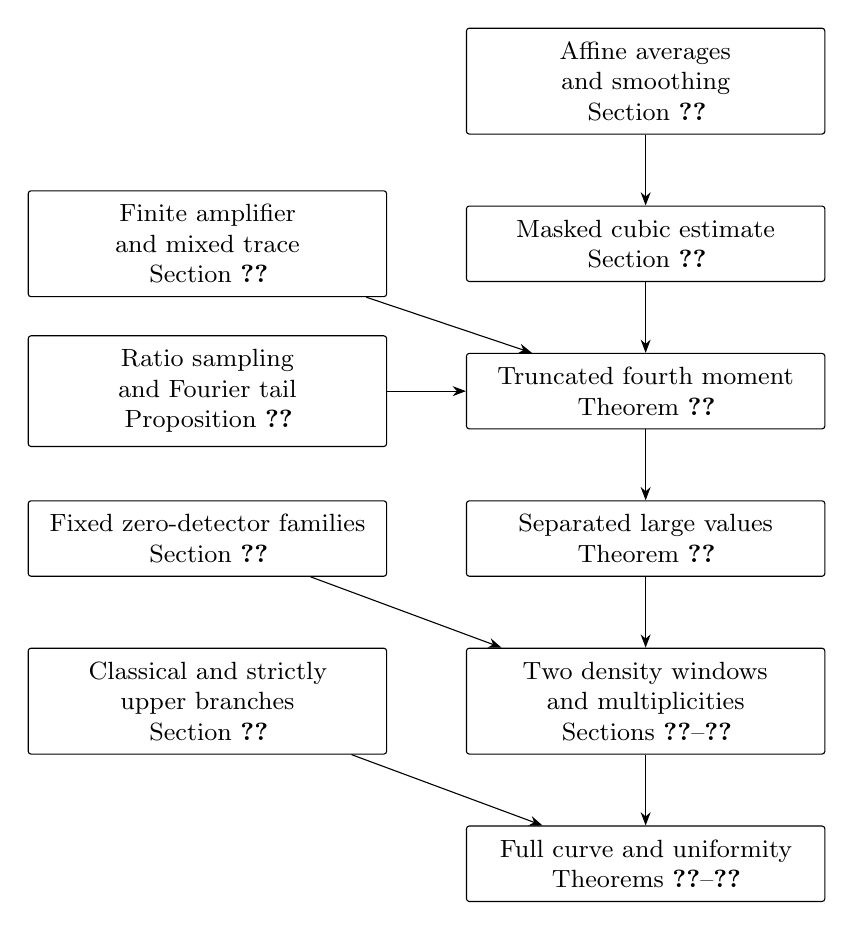
\begin{tikzpicture}[>=Stealth, every node/.style={draw,rounded corners=1pt,align=center,font=\small,text width=4.2cm,inner sep=5pt},node distance=9mm]
\node (aff) {Affine averages and smoothing\\Section~\ref{ch:affine}};
\node[below=of aff] (cub) {Masked cubic estimate\\Section~\ref{ch:cubic}};
\node[left=10mm of cub] (spec) {Finite amplifier and mixed trace\\Section~\ref{ch:cubic}};
\node[below=of cub] (mom) {Truncated fourth moment\\Theorem~\ref{thm:fourth}};
\node[left=10mm of mom] (tail) {Ratio sampling and Fourier tail\\Proposition~\ref{prop:tail}};
\node[below=of mom] (lv) {Separated large values\\Theorem~\ref{thm:middle}};
\node[left=10mm of lv] (det) {Fixed zero-detector families\\Section~\ref{ch:detector}};
\node[below=of lv] (slab) {Two density windows and multiplicities\\Sections~\ref{ch:windows}--\ref{ch:counting}};
\node[left=10mm of slab] (old) {Classical and strictly upper branches\\Section~\ref{ch:otherbranches}};
\node[below=of slab] (full) {Full curve and uniformity\\Theorems~\ref{thm:full}--\ref{thm:away}};
\draw[->] (aff)--(cub);\draw[->] (cub)--(mom);\draw[->] (spec)--(mom);
\draw[->] (tail)--(mom);\draw[->] (mom)--(lv);\draw[->] (lv)--(slab);
\draw[->] (det)--(slab);\draw[->] (slab)--(full);\draw[->] (old)--(full);
\end{tikzpicture}
\caption{The principal analytic and counting dependencies. The classical fourth and twelfth moments are cited at their points of use.}\label{fig:dependencies}
\end{figure}

\subsection{Organization and conventions}
Section~\ref{ch:objects} fixes the zero-count and polynomial conventions. Sections~\ref{ch:affine} and \ref{ch:cubic} develop the affine and spectral estimates. Section~\ref{ch:moment} balances the truncated moment, and Section~\ref{ch:middle} proves Theorem~\ref{thm:middle}. Sections~\ref{ch:detector}--\ref{ch:counting} pass from fixed detector families to the two density windows. Section~\ref{ch:otherbranches} treats the remaining branches. Section~\ref{ch:final} assembles the statements and proves uniformity. An appendix records the precise relation with the registered source and the scope of the analytic citations.

All real integrals use Lebesgue measure. For $x>0$ and real or complex $u$, $x^u=\exp(u\log x)$. Our Fourier transform is
\[
 \widehat h(\xi)=\int_\R h(t)\e^{-2\pi\ii\xi t}\,dt,
 \qquad e(x)=\e^{2\pi\ii x},\qquad\lambda(x)=\frac{\log x}{2\pi}.
\]
For integrable Fourier data, $\mathcal F^{-1}F(t)=\int_\R F(\xi)\e^{2\pi\ii\xi t}\,d\xi$. Plancherel has constant one, and complex inner products are conjugate-linear in the first argument. The notation $\ll$ always allows dependence on parameters explicitly indicated in its subscript and on fixed cutoffs, but not on the displayed varying coefficients, sets or scales. An eventual estimate has a height threshold selected before every variable over which that estimate is uniform. Unless specified otherwise, a polynomial called bounded has $|a_n|\le1$ for $n\in I_N$ only. We write $\tau(n)$ for the divisor function, with $\tau(0)=0$, reserving $d$ for an integer translation in affine sums and $\vartheta$ for the smooth step used in the dyadic partition.

\section{Zero counts and Dirichlet-polynomial conventions}\label{ch:objects}
\subsection{Zeros and analytic multiplicity}
\begin{definition}
Let $\zeta$ be the Riemann zeta function, defined by its Dirichlet series on $\Rea s>1$ and continued meromorphically to $\C$, with its single simple pole at $1$. A nontrivial zero is a complex
number $\rho$ for which
\[
 \zeta(\rho)=0,\qquad 0<\Rea\rho<1.
\]
Define $m(\rho)$ to be the order of vanishing of $\zeta$ at the nontrivial zero $\rho$, as a positive integer. For real $\sigma,a,b$, set
\[
 Z(\sigma;a,b)=\{\rho:\zeta(\rho)=0,\ 0<\Rea\rho<1,\
                  \sigma\le\Rea\rho,\ a\le\Ima\rho\le b\}.
\]
Define the slab and density counts
\[
 n(\sigma;a,b)=\sum_{\rho\in Z(\sigma;a,b)}m(\rho),\qquad
 N(\sigma,T)=n(\sigma;-T,T).
\]
\end{definition}
The zero set is finite, and its multiplicities have their usual analytic meaning.
\begin{lemma}
Every set $Z(\sigma;a,b)$ is finite. At a nontrivial zero, $m(\rho)$ is finite
and positive, and there is an analytic function $g$ near $\rho$, with
$g(\rho)\ne0$, such that locally
\[
 \zeta(z)=(z-\rho)^{m(\rho)}g(z).
\]
\end{lemma}
\begin{proof}
For $\rho\in Z(\sigma;a,b)$, we have
$|\Ima\rho|\le |a|+|b|$ and
\[
 |\rho|\le |\Rea\rho|+|\Ima\rho|\le1+|a|+|b|.
\]
The function $h(z)=(z-1)\zeta(z)$, extended by $h(1)=1$, is entire. Its zeros are therefore isolated, and its zero set in any compact disk is finite: an infinite subset of that disk would have an accumulation point and force $h$ to vanish identically. The zeta zeros in our disk are zeros of $h$, so $Z(\sigma;a,b)$ is finite. Since a nontrivial zero is not the pole, zeta is analytic there. A nonzero analytic function has a finite positive vanishing order at a zero, and its Taylor expansion factors as $(z-\rho)^{m(\rho)}g(z)$ with $g(\rho)\ne0$. Zeta is not identically zero, for instance because $\zeta(2)>0$. These are the usual analytic zero conventions \cite[Chapter~5]{IwaniecKowalski}.
\end{proof}
We record the monotonicity properties used below.
\begin{lemma}
If $\sigma'\le\sigma$, $a'\le a$, and $b\le b'$, then
$n(\sigma;a,b)\le n(\sigma';a',b')$.
\end{lemma}
\begin{proof}
The inequalities on parameters give an inclusion of zero sets. Sum the
nonnegative natural multiplicities over that inclusion.
\end{proof}
For $0\le T\le T'$ and $\sigma'\le\sigma$, the lemma gives $N(\sigma,T)\le N(\sigma',T')$. If $\sigma\ge1$, the count is zero by its definition. Also the number of zero locations in a slab is at most its multiplicity count, since $m(\rho)\ge1$.
\subsection{Polynomial lengths and separation}
\begin{definition}
For $N>0$ put
\[
 I_N=\{n\in\N:\lfloor N\rfloor_+<n\le\lfloor2N\rfloor_+\},\qquad
 D_{N,a}(t)=\sum_{n\in I_N}a_n\e^{\ii t\log(n/N)}.
\]
Here $\lfloor x\rfloor_+=\max(0,\lfloor x\rfloor)$ and $\lceil x\rceil_+=\max(0,\lceil x\rceil)$ for real $x$. For $N>0$, membership in $I_N$ is equivalent to $N<n\le2N$, so this agrees with \eqref{eq:introD}.
A finite set $W\subset\R$ is one-separated if
$|t-u|\ge1$ whenever $t,u\in W$ and $t\ne u$.
\end{definition}
The coefficient hypothesis throughout is $|a_n|\le1$ for $n\in I_N$;
no hypothesis is placed on coefficients outside that interval.
The following comparison permits passage between real and integer lengths.
\begin{lemma}
For $N>0$, the norm of $D_{N,a}$ equals the norm of
$\sum_{n\in I_N}a_n\e^{\ii t\log n}$. For $N\ge2$ and $M=\lfloor N\rfloor_+$,
\[
 M\ge2,\quad N/2\le M\le N,\quad
 \lfloor2N\rfloor_+\in\{2M,2M+1\}.
\]
For bounded polynomial coefficients,
\[
 |D_{N,a}(t)|\le |D_{M,a}(t)|+1.
\]

\end{lemma}
\begin{proof}
Factor out $\e^{-\ii t\log N}$, which has modulus one. The floor inequalities
$M\le N<M+1$ give the bounds on $M$ and the two possible values of
$\lfloor2N\rfloor_+$. The integer sum at real length differs from the sum at
length $M$ by either no term or the term with index $2M+1$. That term has norm
at most one. The triangle inequality proves the comparison. For $V\ge2$, the comparison gives $|D_{M,a}(t)|\ge V-1\ge V/2$ whenever $|D_{N,a}(t)|\ge V$.
\end{proof}
\section{Affine averages, smoothing and Fourier decay}\label{ch:affine}
\subsection{Affine averages and their Fourier profile}
\begin{definition}
For $R,K\ge1$ and $C_0\ge0$, let
\[
 \mathcal B(R,K,C_0)=\{(b,q,d)\in\Z^3:
 R\le|b|\le2R,\ K\le q\le2K,\ |d|\le C_0R\}.
\]
The slope has both signs; the denominator is positive. Put
\[
 J_{R,K,C_0}(g)=\int_\R
 \left(\sum_{(b,q,d)\in\mathcal B(R,K,C_0)}
                  g\left(\frac{bu+d}{q}\right)\right)^2\,du.
\]
For a finite subset $S$ the corresponding energy $J_S(g)$ uses $S$ in the sum.
For a smooth compactly supported input, let
$\|g\|_\infty=\sup_x|g(x)|$.
A fixed Fourier profile $D(\beta,n)$ means the family of bounds
\begin{equation}\label{eq:supprofile}
 |\Hhat g(\xi)|\le D(\beta,n)\mathcal T^\beta
       (\mathcal T/|\xi|)^n\|g\|_\infty
 \quad(\beta>0,\ n\in\N,\ \xi\ne0).
\end{equation}
\end{definition}
We use the following unequal-scale refinement of the affine estimate.
\begin{proposition}\label{input:affine}
Fix $0<a\le b$, $C_0\ge0$, and a nonnegative Fourier profile $D$.
For each $\eps>0$ there is $C>0$ such that for all
$\mathcal T\ge2$, $1\le K\le R\le\mathcal T^4$, and all nonnegative
$C^\infty$ functions $g$ supported in $[a,b]$ satisfying
\eqref{eq:supprofile},
\begin{equation*}
 J_{R,K,C_0}(g)\le C\mathcal T^\eps
 \left(R^2K^4\left(\int g\right)^2+RK^3\int g^2\right).
\end{equation*}

\end{proposition}
The unequal-scale refinement in Proposition~\ref{input:affine} is a theorem of \cite{Lewko}. The balanced-scale estimate and the underlying iterative method are Guth--Maynard's Proposition~9.1 and Lemma~9.2 \cite{GuthMaynard}. We record the reductions and constant selection needed here; the Poisson--divisor recurrence itself is a cited analytic result, not an elementary consequence of Cauchy--Schwarz.
\paragraph{Reduction and finite iteration.}
The following explanation retains the two-stage reduction; it does not
replace this input by an unproved affine conjecture. For positive integer shell sizes $M_1,M_2,M_3$, sum over $M_1\le|m_1|\le2M_1$, $M_2\le|m_2|\le2M_2$, and $|m_3|\le8M_3$. The balanced auxiliary energy $\mathcal J(g,M)$ is the maximum, over integers $1\le M_j\le M$, of the integral of the square of $\sum g((m_1u+m_3)/m_2)$. Here $M$ is a positive integer. The finite maximum is used only for this balanced auxiliary estimate.
The auxiliary recurrence uses a mass-normalized Fourier-height family, different from \eqref{eq:supprofile}:
\[
 \sup_\xi |\xi|^n|\Hhat g(\xi)|
 \le 2^dD(\beta,n)\mathcal T^\beta\mathcal T^{n+2}\int g
\]
at smoothing depth $d\in\N$. The support envelope at that depth is
$[1/4-2d/\mathcal T,\,9/4+2d/\mathcal T]$.
The factor $\mathcal T^{n+2}$ is not a height-independent constant.

The Lemma-9.2 reduction supplies, after choosing its Fourier order,
a recurrence of the form
\begin{equation}\label{eq:affrec}
 \mathcal J(g,M)\le A\mathcal T^\alpha M^6\Bigl(\int g\Bigr)^2
 +B\mathcal T^\alpha M^2\|g\|_2
       \sqrt{\mathcal J(\widetilde g,M_2)}
 +E\Bigl(\int g\Bigr)^2,
 \qquad M_2\le M.
\end{equation}
Here $A,B,E$ are uniform functions of the selected Fourier order, divisor
constant, and current profile. The recurrence includes a nonnegative convolution smoothing $\widetilde g$. Its Fourier multiplier is supplied by the Poisson reduction at parameter $\mathcal T+M_2/(2M_3)$, after division by the first Poisson window; the norm, support and profile properties below are part of that analytic recurrence.
It preserves nonnegativity, enlarges the support by at most $2/\mathcal T$,
and updates the Fourier coefficient by a factor two. The development proves
\[
 M_2^6\Bigl(\int\widetilde g\Bigr)^2+M_2^4\int\widetilde g^2
 \le16\left(M^6\Bigl(\int g\Bigr)^2+M^4\int g^2\right).
\]
Let the latter parenthesis be $W$. For a desired loss $\delta$, choose finitely
many descent steps $r$ with $(3/2)^r\delta\ge100$. At the terminal loss
$\ge100$, the crude bound
$\mathcal J(g,M)\le36992M^6\int g^2$ and $M\le\mathcal T^4$ suffice.
At an induction step use \eqref{eq:affrec} with $\alpha=\delta/8$ and the
induction hypothesis with loss $3\delta/2$ on $\widetilde g$. It gives
\[
 \sqrt{\mathcal J(\widetilde g,M_2)}
 \le4\sqrt{C_{\rm next}}\mathcal T^{3\delta/4}\sqrt W.
\]
Since $M^2\|g\|_2\le\sqrt W$, the mixed term is at most
$4B\sqrt{C_{\rm next}}\mathcal T^{7\delta/8}W$.
The first and last terms are at most $(A+E)\mathcal T^\delta W$; for the last term use $M\ge1$ and hence $(\int g)^2\le W$.
Thus $C=A+E+4B\sqrt{C_{\rm next}}+1$ closes the induction. A threshold
$\mathcal T\ge\max(2,8r)$ guarantees all support envelopes used by this
finite descent. This is why the complete profile must be fixed before the
varying function and height.
The unequal-scale Poisson reduction retains an outer factor $RK$, not a
factor $R^2$. With $m=\int g$ and $n=\|g\|_2$ it supplies
\[
 J\le E_0(R^2K^4m^2+RK n\sqrt Q),\qquad
 Q\le H_0(K^6m^2+K^4n^2),\quad H_0\ge1.
\]
Hence $\sqrt Q\le\sqrt{H_0}(K^3m+K^2n)$. The cross term
$RK^4mn$ is at most $R^2K^4m^2+RK^3n^2$, by expanding a nonnegative
square and using $K\le R$. Therefore
\[
 J\le2E_0\sqrt{H_0}(R^2K^4m^2+RK^3n^2).
\]
The development takes $E_0=A_0\mathcal T^{\eps/2}$ and
$H_0=(B_0+1)\mathcal T^\eps$, so the total loss is exactly
$\mathcal T^\eps$. Heights below $8$ are treated by the crude finite
bound and $R\le8^4$, not discarded.
\paragraph{Exact Poisson normalizations.}
For a Schwartz function $\psi$, scale $R>0$, and real $\alpha$, the identities used in that reduction are
\[
 \Hhat{(\psi(\cdot/R)e(\alpha\cdot))}(\xi)
       =R\Hhat\psi(R(\xi-\alpha)),\qquad
 \sum_{d\in\Z}\psi(d/R)e(\alpha d)
       =R\sum_{\ell\in\Z}\Hhat\psi(R(\ell-\alpha)).
\]
The affine Fourier factor for positive $b,q$ is
$e(\xi d/b)(q/b)\Hhat g(q\xi/b)$. Signed slopes are handled by
explicit reindexing. The Schwartz decay and compact support ensure absolute convergence in the displayed identities; the deeper interchanges inside the cited recurrence use its integrability estimates. Passing from canonical support to general fixed
positive support uses a fixed integer $\ell\ge1$ large enough to contain that support in $[0,\ell]$, the function $g_1(x)=g(\ell(x-1))$, and the injective index map
$(b,q,d)\mapsto(b,\ell q,d+\ell q)$; there is no Jacobian in $u$.
\subsection{Smoothing restricted densities}
Let $b_\kappa$ be the fixed smooth nonnegative bump centered at zero, equal to $1$ on $[-1,1]$ and zero outside $[-2,2]$. Its normalized kernel is the exact function
$\kappa(x)=b_\kappa(x)/\int b_\kappa$; the denominator is strictly positive.
Thus $\kappa$ is nonnegative, compactly supported, smooth and has mass one.
Set $\kappa_h(x)=h^{-1}\kappa(x/h)$ and $S_hg=\kappa_h*g$, for $h>0$.
Smoothing preserves mass and contracts the square norm.
\begin{lemma}
For nonnegative integrable $g$ with $g^2$ integrable,
\[
 \int S_hg=\int g,\qquad \int(S_hg)^2\le\int g^2.
\]
If $g$ is supported in $[a,b]$, $S_hg$ is smooth and supported in
$[a-2h,b+2h]$.
\end{lemma}
\begin{proof}
Tonelli and the mass-one identity give preservation of mass. Apply the
weighted Cauchy--Schwarz inequality at each $x$ to
$\int\kappa_h(y)g(x-y)\,dy$, then integrate and use translation invariance.
The support inclusion follows because $x-y$ cannot be in $[a,b]$ when
$x$ is outside its $2h$ enlargement and $|y|\le2h$. Derivatives may be taken on the compactly supported smooth convolution factor: each derivative is bounded and compactly supported, so dominated convergence against the integrable input gives the derivative of the convolution.
\end{proof}
The affine estimate remains valid after restricting a density to an arbitrary measurable set.
\begin{proposition}\label{prop:maskedaff}
Fix $0<a\le b$ and $C_0\ge0$. For each $\eps>0$ one constant works for
all admissible $\mathcal T,R,K,h$, every measurable set $E$, and every
measurable real $r$ supported in $[a,b]$ with $r^2,r^4$ integrable:
\[
 J_{R,K,C_0}\bigl(S_h(\one_Er^2)\bigr)
 \le C\mathcal T^\eps
 \left(R^2K^4\Bigl(\int_Er^2\Bigr)^2+RK^3\int_Er^4\right),
\]
where $\mathcal T\ge2$, $1\le K\le R\le\mathcal T^4$, and
$0<h\le\min(1,a/4)$, $h^{-1}\le\mathcal T$.
\end{proposition}
\begin{proof}
The smoothed function is nonnegative, smooth, and supported in
$[a/2,b+2]$. Put $g=\one_Er^2$ and $F_h=\kappa_h*g$. Fourier convolution and the decay of $\widehat\kappa$ give $|\xi|^j|\widehat F_h(\xi)|\le C_jh^{-j}\int g$. By mass preservation and the support bound,
\[
 \int g=\int F_h\le(b-a+4h)\|F_h\|_\infty\le(b-a+4)\|F_h\|_\infty.
\]
Since $h^{-1}\le\mathcal T$ and $\mathcal T^\beta\ge1$, this gives \eqref{eq:supprofile} with a fixed profile independent of $E,r,h,\mathcal T$. This argument also covers zero mass, and never divides by the mass. Apply Proposition~\ref{input:affine} on the enlarged fixed
interval. The preceding lemma preserves $\int_Er^2$ and bounds the output
square integral by $\int_Er^4$. This proves the assertion including the
case of zero restricted mass. No regularity of the boundary $\partial E$ is used.
\end{proof}
\section{Centered kernels and spectral comparison}\label{ch:cubic}
\subsection{Kernels and phase operators}
Fix the comparison bump $w$: it is the smooth bump centered at $5/2$
with inner radius $3/2$ and outer radius $2$. Thus $0\le w\le1$,
$w=1$ on $[1,4]$, and its closed support is contained in $[1/2,5]$.
Put $a_0(x)=w(x)^2$ and $\chi(s)=w(s+2)$.
Then $0\le\chi\le1$, $\chi=1$ on $[-1,2]$, and
$\supp\chi\subset[-2,3]$.
For $L>0$ and a smooth amplitude $a$ supported in $[l,u]\subset(0,\infty)$ define
\begin{equation}\label{eq:kernel}
 K_{a,L}(s)=\sum_{\lceil lL\rceil\le m\le\lfloor uL\rfloor}
             a(m/L)\e^{\ii s\log(m/L)}
           -L\int_\R a(x)\e^{\ii s\log x}\,dx.
\end{equation}
For a measurable nonnegative integrable time density $\mu$, set
$d\nu_\mu(t)=\mu(t)\,dt$ and
\[
 \mathcal C_{a,L}(\mu)=\iiint
 K_{a,L}(t_1-t_2)K_{a,L}(t_2-t_3)K_{a,L}(t_3-t_1)
 \prod_{j=1}^3d\nu_\mu(t_j).
\]
The triple integral is defined before it is identified with an operator trace.
In $\mathcal H=L^2(\nu_\mu;\C)$, let
$p_x(t)=e(t\lambda(x))$. For a real nonnegative cutoff $a$, define
\[
 G=\sum_{\lceil lL\rceil\le m\le\lfloor uL\rfloor}
 a(m/L)\,p_{m/L}\otimes p_{m/L},\qquad
 C=L\int a(x)\,p_x\otimes p_x\,dx,\qquad H=G-C.
\]
Here $(v\otimes v)z=\langle v,z\rangle v$.
An operator $A$ is positive if it is self-adjoint and $\langle v,Av\rangle\ge0$ for all $v$. The operators $G,C$ are positive, while $H$ need not be positive. A nuclear (trace-class) presentation here is a sum or integral of rank-one operators with finite integral of the product of the two vector norms. For a countable orthonormal basis $b=(b_j)$ define $\tr_b A=\sum_j\langle b_j,Ab_j\rangle$ for such an operator. The sum is absolutely convergent and independent of the basis.
The development constructs the integral as a nuclear integral of rank-one operators;
$\int\|La(x)p_x\|\|p_x\|\,dx<\infty$ follows from $a\in L^1$ and
$\|p_x\|^2=\nu_\mu(\R)$.
The centered cubic is an operator trace.
\begin{lemma}
For a countable Hilbert basis $b$ of $\mathcal H$,
\[
 \tr_b(H^3)=\mathcal C_{a,L}(\mu)
\]
for the nuclear operators used here.
\end{lemma}
\begin{proof}
Expand the nuclear presentations of the three factors. A rank-one cyclic
product has trace the cyclic product of three feature inner products.
Since $\langle p_x,p_y\rangle=\Hhat\mu(\lambda(x)-\lambda(y))$ with the
our Fourier convention, integration over frequencies gives the Fourier-side
cyclic product; Fubini gives the independently defined time-side kernel
cubic. The discrete-continuous difference is represented by the disjoint
union of finite counting frequencies and continuous frequencies, with signed
amplitude. Absolute integrability of the products is bounded by the product
of the nuclear norm integrals. This justifies the expansion and every
interchange. The development proves basis-independence through these integral
presentations, rather than presuming an infinite eigenbasis.
\end{proof}
\subsection{The cubic estimate with a restricted Fourier factor}
For the remainder of this section $\mu\ge0$ is measurable, belongs to
$L^1\cap L^2$, and is supported in an interval of length at most $\mathcal T$.
For a measurable Fourier set $B\subset\R$, write
\[
 F=\Hhat\mu,\quad M=\int\mu^2,\quad M_1=\int\mu,\quad
 E=\int|F|^4,\quad E_0=\int_{B^c}|F|^4,\quad A_2=\int_B|F|^2.
\]
The Fourier square and fourth powers are integrable: Plancherel gives
$\int|F|^2=M$, and $|F|\le M_1$ gives
$\int|F|^4\le M_1^2M$.

The key estimate retains a restricted Fourier square mass.
\begin{proposition}\label{input:maskedcubic}
For fixed smooth $a$ supported in a fixed positive interval, each $\eps>0$
has a constant $C>0$ such that if
$\mathcal T\ge2$, $\mathcal T^{4/5}\le L\le\mathcal T$, and $B$ is
measurable and symmetric under $\xi\mapsto-\xi$, then
\begin{equation}\label{eq:maskedcubic}
 |\mathcal C_{a,L}(\mu)|\le C\mathcal T^\eps
 \left(\mathcal T^2M^{3/2}+\mathcal TL\sqrt M\sqrt{E_0}
    +\sqrt{A_2}(\mathcal T^2M+\mathcal TL\sqrt E)\right).
\end{equation}

\end{proposition}
Proposition~\ref{input:maskedcubic} is the masked extension proved in \cite{Lewko}; its proof follows the ratio-coordinate and affine method of \cite[Sections~7--9]{GuthMaynard}. In particular, the restricted factor is part of the stated result and cannot be discarded. We give the precise reduction used in the moment argument.
\paragraph{Poisson reduction of the cubic.}
Poisson summation turns \eqref{eq:kernel} into the sum of the nonzero modes
$L\Hhat{(a(x)\e^{\ii s\log x})}(Lm)$. The development retains
$0<|m|\le U$, $U=\mathcal T^{1+\eta}/L$, choosing $0<\eta<4/5$ before
all varying data. It bounds the cubic replacement error by
$C\mathcal T^{-100}M^{3/2}$. Expanding the retained cube gives the exact
factor $L^3$ and, for $m=(m_1,m_2,m_3)$, the spatial integral with amplitude
$a(x_1)a(x_2)a(x_3)$, phase $e(-L(m_1x_1+m_2x_2+m_3x_3))$, and Fourier product
\[
 F(\lambda(x_3)-\lambda(x_1))
 F(\lambda(x_1)-\lambda(x_2))
 F(\lambda(x_2)-\lambda(x_3)).
\]
Set $x_1=rv$, $x_2=ry$, $x_3=r$. The Jacobian is exactly $r^2$.
The Fourier product becomes
$F(-\lambda(v))F(\lambda(v)-\lambda(y))F(\lambda(y))$.
Radial integration, before taking a norm, yields rapid decay in
$L(m_1v+m_2y+m_3)$. The near region is the thin strip
$|L(m_1v+m_2y+m_3)|\le\mathcal T^\eta$.
It is rewritten as a window of width
$\mathcal T^\eta/(L|m_2|)$ about
$-(m_1v+m_3)/m_2$. Negative denominators are normalized by simultaneous
negation of modes. For the inverse-ratio energy, the exact identity
\[
 \frac{-(m_1v+m_3)/m_2}{v}
 =-\frac{m_3/v+m_1}{m_2}
\]
swaps slope and translation. The Jacobian for $v\mapsto1/v$ is bounded on
the fixed positive ratio interval (the ratios of points in the fixed support of $a$). Both energies use the mixed-box version of Proposition~\ref{prop:maskedaff}, proved in \cite{Lewko}. A slope shell $B_0\le|b|\le2B_0$ and a positive denominator shell $Q_0\le q\le2Q_0$ may be independent, while $|d|\le C_0R$; if $1\le B_0\le R$, $1\le Q_0\le K\le R$, the bound is $\mathcal T^\eps(R^2K^4m^2+RK^3n^2)$ with the restricted mass $m$ and square norm $n$. For the original strip use slope $-m_1$, denominator $m_2$ and translation $-m_3$; for the inverse ratio use slope $-m_3$, the same denominator $m_2$, and translation $-m_1$. Both numerators have shell sizes at most $R$, and the denominator shell is $K$. No minimum of the three shell sizes is asserted. This independent-shell version is part of the cited affine theorem, not a relabelling that changes the denominator. The dyadic mode sum,
width losses, mode count, and radial discard are included in the estimates below. In Fourier coordinates the relevant
measure change is $dx=2\pi x\,d\lambda$; no unrecorded normalization change
is made.

For a symmetric exceptional set $B$, the retained cubic is partitioned exactly
into four integrals, after cyclic reindexing, with masks
\[
 (B^c,B^c,B^c),\qquad(B,\R,\R),\qquad
 (B,\R,B^c),\qquad(B,B^c,B^c).
\]
Before reindexing, the disjoint partition is $(B^c,B^c,B^c)$, $(B,\R,\R)$, $(B^c,B,\R)$, and $(B^c,B^c,B)$. Cyclic reindexing of both spatial coordinates and the full mode cube gives the displayed four integrals, with the exceptional mask always in the first factor. They are an equality of integrals after reindexing, not four pointwise disjoint sets in their final displayed positions. The term with no exceptional Fourier factor costs
$\mathcal T^\eps(\mathcal T^2M^{3/2}+\mathcal TL\sqrt M\sqrt{E_0})$;
each of the other three costs
$\mathcal T^\eps\sqrt{A_2}(\mathcal T^2M+\mathcal TL\sqrt E)$.
The homogeneous negligible errors are absorbed by the first term.
For bounded heights the development separately bounds the cubic by a constant
multiple of $\mathcal T^2M^{3/2}$. Thus eventual Poisson retention is not
used to skip the bounded-height range.
\paragraph{Explicit affine-to-cubic exponent estimate.}
For fixed ratio support and a fixed factor $q_0\ge1$, the smoothing width
in a denominator shell $K$ is $h=q_0\mathcal T^\eta/(LK)$.
For $1\le K\le R\le U=\mathcal T^{1+\eta}/L$ one has
$h^{-1}\le\mathcal T$ and
$h\le q_0\mathcal T^{\eta-4/5}$. Since $\eta<4/5$, a single eventual
height threshold puts every such width in the admissible compact-smoothing
range of Proposition~\ref{prop:maskedaff}.
After the affine estimate and Cauchy--Schwarz, a box contribution at restricted
first-factor square mass $A$ and other-factor masses $M_D,E_D$ has scalar factor
\[
 \sqrt A\frac{L^2\mathcal T^\eta}{K}
       \sqrt{R^2K^4M_D^2+RK^3E_D}.
\]
The square root is at most $K(RKM_D+\sqrt{RK}\sqrt{E_D})$.
Both $RK\le U^2$ and $\sqrt{RK}\le U$; hence the factor is at most
\[
 \sqrt A\left(\mathcal T^{3\eta}\mathcal T^2M_D
                +\mathcal T^{2\eta}\mathcal TL\sqrt{E_D}\right),
\]
because $L^2\mathcal T^\eta U^2=\mathcal T^{2+3\eta}$ and
$L^2\mathcal T^\eta U=\mathcal T^{1+2\eta}L$.
A Fourier-affine loss $\mathcal T^\alpha$ contributes
$\mathcal T^{\alpha/2}$ after the square root. The finite dyadic-class
count contributes at most $D_\delta\mathcal T^\delta$, since $U\le\mathcal T$.
Choose $\eta=\min(\eps/12,1/10)$, $\alpha=\eps/4$, $\delta=\eps/4$;
then $\delta+\alpha/2+3\eta\le\eps$.
Thus both terms fit the displayed masked-cubic bound while the restricted
factor $\sqrt A$ is retained unchanged. Passing back from ratio coordinates
charges only fixed factors bounded using $dx=2\pi x\,d\lambda$.
A Fourier threshold gives a useful consequence of the preceding proposition.
\begin{proposition}\label{prop:restricted}
For the same $a,\mu,\mathcal T,L$ and every $\Lambda\ge0$,
\begin{equation*}
 |\mathcal C_{a,L}(\mu)|\le C\mathcal T^\eps
  \left(\mathcal T^2M^{3/2}+\mathcal TL\Lambda M
       +\mathcal TL M_1\int_{\{|F|>\Lambda\}}|F|^2\right).
\end{equation*}
\end{proposition}
\begin{proof}
Take $B=\{|F|>\Lambda\}$. The Fourier transform is continuous, so $B$ is
measurable. Because $\mu$ is real, $F(-\xi)=\overline{F(\xi)}$, so $B$ is
symmetric. Put $A_2=\int_B|F|^2$. Plancherel and the pointwise bounds give
\[
 A_2\le M,\qquad E_0\le\Lambda^2M,\qquad
 E\le\Lambda^2M+M_1^2A_2.
\]
It follows that $\mathcal TL\sqrt M\sqrt{E_0}\le\mathcal TL\Lambda M$
and $\mathcal T^2M\sqrt{A_2}\le\mathcal T^2M^{3/2}$.
Also $\sqrt E\le\Lambda\sqrt M+M_1\sqrt{A_2}$; hence
\[
 \mathcal TL\sqrt{A_2}\sqrt E
 \le\mathcal TL\Lambda M+\mathcal TL M_1A_2.
\]
Substituting these three inequalities in \eqref{eq:maskedcubic} increases its
constant by at most a factor three. This includes zero mass and zero threshold.
\end{proof}
\subsection{The divisor amplifier and spectral inequality}
The amplifier column set is
\[
 Q_{N,L}=\{q\in\N:\lceil L/N\rceil_+\le q\le\lfloor2L/N\rfloor_+\}.
\]
For $N>0$, $N\le L$, its cardinality $k$ satisfies
$L/(2N)\le k\le2L/N$. Its divisor matrix is
\[
 B_{m,q}=\sum_{n\in I_N}\one_{m=qn}a_n.
\]
Every contributing product $qn$ has $1\le qn/L\le4$, the plateau of $w$.
Its synthesized column, obtained by summing against $w(m/L)p_{m/L}$ over the integer rows, is exactly
$\e^{\ii t\log(qN/L)}D_{N,a}(t)$.
The development bounds the amplifier norm by divisor multiplicity, using the
established subpower divisor bound $\tau(n)\ll_\eta n^\eta$.
It then constructs a finite orthonormal family in its synthesized range,
not a postulated infinite eigenfamily.
The finite amplifier gives an orthonormal family with a quadratic lower bound.
\begin{proposition}\label{input:amp}
For each $\eta>0$ there is $P>0$ such that, uniformly in the bounded
coefficients, scales $N>0$, $N\le L$, and measurable nonnegative integrable time densities $\mu$,
there is an orthonormal family $v_1,\ldots,v_r$, $r\le k$, satisfying
\[
 k\frac{\int\mu|D_{N,a}|^2}{P(1+L)^\eta(N+1)}
 \le\sum_{j=1}^r\langle v_j,Gv_j\rangle.
\]
Here $G$ uses amplitude $w^2$ on the indicated integer rows.

\end{proposition}
\begin{proof}
Let $\mathsf A$ be the divisor matrix between the finite column
and row Euclidean spaces. For a row $m$, the set of factorizations is
$F_m=\{(q,n)\in Q_{N,L}\times I_N:qn=m\}$.
Cauchy--Schwarz and $|a_n|\le1$ give
$|\mathsf A z(m)|^2\le|F_m|\sum_{(q,n)\in F_m}|z_q|^2$.
A nonempty factorization set injects into the divisors of $|m|$ and has $0<m\le4L$.
Thus $|F_m|\le C_\eta(1+L)^\eta$. Summing over rows counts each $(q,n)$
at most once and gives
$\|\mathsf A\|^2\le P(1+L)^\eta(N+1)$.
Let $\mathcal B$ synthesize a row coordinate into $w(m/L)p_{m/L}$.
Then $\mathcal B\mathcal B^*=G$ exactly. Every synthesized column
$\mathcal B\mathsf A e_q$ has square norm $\int\mu|D|^2$ by the
plateau identity and its unit phase.
Choose an orthonormal basis $v_1,\ldots,v_r$ of the finite range of
$\mathcal B\mathsf A$; $r\le k$. Parseval in that range and adjoint
Parseval in the finite column space give
\[
 \sum_q\|\mathcal B\mathsf A e_q\|^2
 =\sum_j\|\mathsf A^*\mathcal B^*v_j\|^2
 \le\|\mathsf A\|^2\sum_j\|\mathcal B^*v_j\|^2
 =\|\mathsf A\|^2\sum_j\langle v_j,Gv_j\rangle.
\]
Insert the matrix bound and divide by its positive uniform upper bound.
This proves the asserted orthonormal-family bound, including rank zero.
\end{proof}
For the continuous operator, let $c_{a_0}(s)=\int a_0(x)\e^{\ii s\log x}\,dx$. With $x=\e^y$, this is the Fourier transform, up to our normalization, of a compactly supported smooth function of $y$, and therefore $c_{a_0}\in L^1(\R)$. Its kernel is $Lc_{a_0}(t-u)$. If $0\le\mu\le B$, then
\[
 \sup_t\int L|c_{a_0}(t-u)|\mu(u)\,du\le LB\|c_{a_0}\|_1,
\]
and the same bound holds with $t,u$ exchanged. Schur's inequality gives $\|C\|\le D_0LB$, with $D_0=\|c_{a_0}\|_1$ depending only on the fixed cutoff.

Write $x_+=\max(x,0)$ for real $x$. Positivity of the two comparison operators controls the negative eigenvalues of their difference.
\begin{lemma}
If $C\ge0$ and $G=C+H\ge0$ in finite dimension, with $H$ self-adjoint and eigenvalues $h_j$
of $H$, then
\[
 \sum_j(h_j)_+^3\le|\tr(H^3)|+\tr(CH^2).
\]
\end{lemma}
\begin{proof}
In an orthonormal eigenbasis of $H$ put $c_j=\langle b_j,Cb_j\rangle$.
Positivity gives $c_j\ge0$ and $c_j+h_j\ge0$. If $h_j\le0$,
$(-h_j)^3\le c_jh_j^2$; otherwise the left side is zero. Sum these
inequalities. Finally $(h_j)_+^3=h_j^3+(-h_j)_+^3$ and
$\sum h_j^3\le|\sum h_j^3|$. Notice that $C$ is not assumed to commute
with $H$ or to be diagonal.
\end{proof}
The spectral comparison has the following trace-class form.
\begin{proposition}\label{input:spectral}
Let $G,C$ be positive trace-class operators on a separable complex Hilbert space, let $b$ be a countable orthonormal basis, let $k,a,B\ge0$, and let $v_1,\ldots,v_r$ be an orthonormal family with $r\le k$. If $ka\le\sum_{j=1}^r\langle v_j,Gv_j\rangle$ and $\|C\|\le B$, then
\[
 k(a-B)_+^3\le|\tr_b((G-C)^3)|+\Rea\tr_b(C(G-C)^2).
\]

\end{proposition}
\begin{proof}
In finite dimension put $H=G-C$ and let $h_i$ be its eigenvalues in an orthonormal eigenbasis $b_i$. The orthonormal-family hypothesis gives $k(a-B)\le\sum_{j=1}^r\langle v_j,Hv_j\rangle$. Set $w_i=\sum_{j=1}^r|\langle b_i,v_j\rangle|^2$. Bessel and Parseval give $0\le w_i\le1$ and $\sum_iw_i=r\le k$. If $a\le B$ the conclusion is immediate. Otherwise H\"older gives
\[
 k(a-B)\le\sum_iw_i(h_i)_+
 \le\Bigl(\sum_iw_i\Bigr)^{2/3}
     \Bigl(\sum_iw_i(h_i)_+^3\Bigr)^{1/3}
 \le k^{2/3}\Bigl(\sum_i(h_i)_+^3\Bigr)^{1/3}.
\]
For $k>0$, cubing and cancellation, followed by the sign-control lemma, proves the assertion. If $k=0$, the left side is zero and the right side is nonnegative.

For the Hilbert space, take finite-rank orthogonal projections whose ranges contain the orthonormal family and increasingly many vectors of a countable orthonormal basis. The compressions $G_n,C_n$ remain positive, retain the orthonormal-family inequality, and have $\|C_n\|\le B$. Trace-class approximation gives $G_n\to G$ and $C_n\to C$ in trace norm. For example, approximate a trace-class operator by a finite-rank operator first, and then use strong convergence of the projections on that finite-dimensional range. The trace-ideal product inequality $\|AB\|_1\le\|A\|_1\|B\|$ and its reversed version show, by telescoping products, that $\tr(H_n^3)\to\tr(H^3)$ and $\tr(C_nH_n^2)\to\tr(CH^2)$. Passing to the limit proves the inequality. The mixed trace is nonnegative since $\tr(CH^2)=\tr(HCH)$ and $HCH$ is positive. These trace-ideal facts are also realized by the nuclear presentations in \cite{Lewko}.
\end{proof}
The mixed trace is bounded using polynomial domination.
\begin{proposition}\label{input:mixed}
Fix $A\ge1$ and $p>0$. For every $\eps>0$ one constant works whenever
$N\ge2$, $N\le L$, $0\le\mathcal T\le AN^p$, $\mu\in L^1\cap L^2$
is measurable and nonnegative, supported in an interval of length
$\mathcal T$, with bounded coefficients and $\mu\le|D_{N,a}|^2$:
\[
 |\tr_b(CH^2)|\le R_0N^\eps L^2N\mathcal T\int\mu^2.
\]
\end{proposition}
The development discharges this with the following row and cycle bounds.
For a fixed real nonnegative smooth cutoff $v$ supported in $[1/2,5]$, put
$c_v(s)=\int v(x)\e^{\ii s\log x}dx$ and $K=K_{v,L}$.
The polynomial-dominated row theorem of \cite{Lewko}, with these same scale and density hypotheses, states uniformly for $u$ on the time support,
\[
 \int\mu(t)|K(u-t)|^2dt\le R_vN^\eps LN\mathcal T.
\]
Its proof uses the reflected Mellin kernel: near rows use bounded
coefficient/product energy, signed shells use Fourier-reflected band estimates,
and finite dyadic summation includes negative reflection. It applies to the
centered row, not to an unrelated absolute kernel.
The continuous correction has kernel $Lc_v$. The development proves
$\psi=|c_v|\in L^1$, bounded, by compact-smooth Mellin decay.
By the nuclear mixed trace identity its cycle is
\[
 \iiint Lc_v(u-v)K(v-t)K(t-u)\mu(u)\mu(v)\mu(t)\,du\,dv\,dt.
\]
Use $|K(-s)|=|K(s)|$ and
$|K(v-t)K(t-u)|\le(|K(v-t)|^2+|K(u-t)|^2)/2$.
The row bound controls the inner $t$ integral by $R_vN^\eps LN\mathcal T$.
The remaining double integral of $\psi(u-v)\mu(u)\mu(v)$ is at most
$\|\psi\|_1\int\mu^2$, by Young's inequality, $\|\psi*\mu\|_2\le\|\psi\|_1\|\mu\|_2$, followed by Cauchy--Schwarz.
This proves the mixed estimate with constant
$(1+\|\psi\|_1)R_v$. In the raw spectral application $v=a_0=w^2$,
which is itself an admissible reflection cutoff; hence the displayed
$G,C,H$ are exactly the ones in the row estimate.
We now combine the amplifier and the two trace estimates.
\begin{proposition}\label{prop:spectralraw}
Under the hypotheses of Proposition~\ref{input:mixed} and also
$\mu\le\min(|D_{N,a}|^2,B)$, $B\ge0$, let $M=\int\mu^2$.
For any $\eta,\eps>0$ the development supplies constants $P,D_0,R_0>0$ such that
\begin{equation}\label{eq:spectralraw}
 M^3\le4\bigl(P(1+L)^\eta(N+1)\bigr)^3
 \left((D_0LB)^3+\frac{2N}{L}
   \left(|\mathcal C_{a_0,L}(\mu)|+R_0N^\eps L^2N\mathcal T M\right)\right).
\end{equation}
\end{proposition}
\begin{proof}
Pointwise $\mu^2\le\mu|D|^2$, with both integrals justified by boundedness
of the finite polynomial. The amplifier orthonormal family therefore gives a level at
least $M/P_1$, where $P_1=P(1+L)^\eta(N+1)>0$.
Use Proposition~\ref{input:spectral}, $k\ge L/(2N)$, the Schur bound
$\|C\|\le D_0LB$, the cubic trace identity, and Proposition~\ref{input:mixed}.
Writing $z=(M/P_1-D_0LB)_+$ gives
\[
 \frac L{2N}z^3\le|\mathcal C|+R_0N^\eps L^2N\mathcal T M.
\]
Since $M/P_1\le D_0LB+z$ and
$(x+y)^3\le4(x^3+y^3)$ for nonnegative $x,y$, multiplication by $P_1^3$
gives exactly \eqref{eq:spectralraw}. This proof also works when $M=0$.
\end{proof}
The prefactor can be absorbed into an arbitrarily small power of the polynomial length.
\begin{proposition}\label{prop:spectralscale}
Fix $A\ge1$, $p>0$. For every $\delta>0$, one constant $S>0$ works for
$N\ge2$, $N\le L\le AN^p$, $0\le\mathcal T\le AN^p$, and the preceding
densities $\mu$ with $\mu\le\min(|D_{N,a}|^2,B)$ and $B\ge0$:
\begin{equation*}
 M^3\le SN^\delta\left((NLB)^3+\frac{N^4}{L}|\mathcal C_{a_0,L}(\mu)|
                         +N^5L\mathcal T M\right).
\end{equation*}
\end{proposition}
\begin{proof}
Take $\eta=\delta/(6p)$ and the mixed-trace loss $\eps=\delta/2$.
Then $3p\eta+\eps=\delta$. From
$1+L\le(1+A)N^p$ and $N+1\le2N$,
\[
 4\bigl(P(1+L)^\eta(N+1)\bigr)^3N^\eps
 \le32P^3(1+A)^{3\eta}N^{\delta+3}.
\]
Insert an additional $N^\eps\ge1$ in the nonnegative terms of
\eqref{eq:spectralraw} where necessary. Expanding $N^3$ into the three
terms yields $(NLB)^3$, $2N^4|\mathcal C|/L$, and
$2R_0N^5L\mathcal TM$. A uniform constant
$32P^3(1+A)^{3\eta}(D_0^3+2+2R_0)$ dominates their coefficients.
\end{proof}
\section{Truncation and the fourth-moment estimate}\label{ch:moment}
\subsection{The truncated density}
For $N\ge2$, $T>0$, a bounded polynomial $D=D_{N,a}$, and real $U$, put
\[
 \beta_T(t)=\chi(t/T),\qquad
 \mu_U(t)=\one_{\{|D(t)|\le U\}}\beta_T(t)|D(t)|^2,\qquad
 r_U(t)=\one_{\{|D(t)|>U\}}\beta_T(t)|D(t)|^2.
\]
The measure density is \emph{discarded} above $U$; it is not
$\min(|D|^2,U^2)$. Let
\[
 M=\int\mu_U^2,\qquad H_{\rm rem}=\int r_U,\qquad M_1=\int\mu_U.
\]
All these integrals are finite and nonnegative. Indeed $D$ is a finite
continuous sum with $|D|\le N+1\le2N$ and $\beta_T$ is bounded and
compactly supported. The development proves measurability and integrability of
$\mu_U$, $\mu_U^2$, and $r_U$, support in $[-2T,3T]$, and
\[
 0\le\mu_U(t)\le\min(|D(t)|^2,U^2),\qquad
 \mu_U+r_U=\beta_T|D|^2.
\]
For negative $U$, $\mu_U=0$; the domination statement remains valid.
\subsection{Primitive-ratio sampling and the Fourier tail}
We use the following sampling estimate for logarithmic ratios.
\begin{proposition}\label{input:sampling}
For the fixed $\chi$, one $D_0>0$ works for all $N,T\ge2$ and bounded
polynomial coefficients. For every complex test $h$ with $h\in L^1\cap L^2$,
$\Hhat h\in L^1$, and $\supp h\subset\supp\beta_T$,
\[
 \left|\int |D(t)|^2h(t)\,dt\right|
 \le D_0N^2\int|\Hhat h|+
      D_0N\sqrt{T\log(2N)}\left(\int|h|^2\right)^{1/2}.
\]
\end{proposition}
Proposition~\ref{input:sampling} is the primitive-ratio estimate proved in \cite{Lewko}. Its arithmetic decomposition and scalar summation are as follows.
\paragraph{Primitive ratios and sampling.}
Expansion of $|D|^2$ reduces pairing to Fourier samples at
$\log(n/m)/(2\pi)$, $n,m\in I_N$. Reduce $(n,m)$ by its greatest common
divisor to $(a,b)$; its multiplicity is the number of pairs on that
primitive rational ray. It is at most $\lfloor2N\rfloor/\max(a,b)$.
The height of a pair $(a,b)$ is $\max(a,b)$. Distinct primitive pairs of height at most $Y$ have logarithms separated
by at least $Y^{-2}$: their integer cross-products differ by at least one,
and $\log p-\log q\ge1/p$ for $p\ge q+1$. Thus the Fourier frequencies, which include division by $2\pi$, are separated by $(2\pi Y^2)^{-1}$.
At height $q$ there are at most $2q$ positive pairs. Thus squared
multiplicities through height $Y$ have sum at most
$2\lfloor2N\rfloor^2(1+\log Y)$.
Let $F_h=\widehat h$. Compact time support gives differentiability and $F_h'=\mathcal F(-2\pi\ii t h)$. Plancherel implies $\|F_h'\|_2\le2\pi cT\|h\|_2$ when $\supp h\subset[-cT,cT]$. At $\Delta$-separated points $x_j$, use the disjoint intervals $(x_j,x_j+\Delta]$. The fundamental theorem of calculus, integrated over those intervals, gives
\[
 \sum_j|F_h(x_j)|\le\Delta^{-1}\int_A|F_h|+\int_A|F_h'|,
\]
where $A$ contains those intervals. Applied to $|F_h|^2$ on the whole line, it gives
\[
 \sum_j|F_h(x_j)|^2
 \le\Delta^{-1}\|h\|_2^2+2\|F_h\|_2\|F_h'\|_2
 \le(\Delta^{-1}+4\pi cT)\|h\|_2^2.
\]
The variation bound follows since $|(|F_h|^2)'|\le2|F_hF_h'|$. These are the point-sampling estimates implemented in \cite{Lewko}. Weighted Cauchy--Schwarz with the sum of squared ray multiplicities gives the low-height estimate below. In a dyadic height shell $Q<\max(a,b)\le2Q$, the ray weight is at most $2N/Q$ and frequency separation at least $(8\pi Q^2)^{-1}$. Their sampling intervals lie in $[-2,2]$ for $Q\ge2$, because $n,m\in I_N$ give $|\lambda(n/m)|\le\log2/(2\pi)$. The first displayed variation bound and Cauchy--Schwarz on this fixed band give the high-shell estimate below. Thus the diagonal ratio, repeated ratios and nonintegral endpoints are all retained.
More precisely, set $Y=\min(2N,\max(2,\sqrt T))$ and choose the least $J$
with $2N\le2^JY$. Then $Y\ge2$, $Y^2\le2T$,
$\sum_{j<J}2^jY\le4N$ and $\sum_{j<J}(2^jY)^{-1}\le2/Y$.
If $Y=2N$ then $J=0$; otherwise $Y\ge\sqrt T$.
For a test supported in $[-cT,cT]$, with
$M_h=\int|h|^2$ and $I_h=\int_{-2}^2|\widehat h|$, the exact low-height
sampling cost is at most
\[
 \sqrt{16N^2\log(2N)}\sqrt{(2\pi Y^2+4\pi cT)M_h}.
\]
The established shell-variation bound at height $Q=2^jY$ is
$16\pi NQI_h+8\pi NcTQ^{-1}\sqrt{M_h}$.
The geometric sums therefore give high cost at most
$64\pi N^2I_h+16\pi c(NT/Y)\sqrt{M_h}$, with the second term absent
when $J=0$. Since $NT/Y\le N\sqrt T$ when it is present, and
$\log(2N)\ge1$, the low and high terms fit
\[
 (64\pi+8\sqrt{\pi(1+c)}+16\pi c)
      \left(N^2I_h+N\sqrt{T\log(2N)}\sqrt{M_h}\right).
\]
For the fixed time support take $c=3$ and enlarge the band integral to the
full Fourier $L^1$ integral. The finite expansion of the polynomial pairing
then gives Proposition~\ref{input:sampling}, with bounded coefficients applied
only inside $I_N$.
The Fourier square mass above the removal-dependent threshold is controlled uniformly.
\begin{proposition}\label{prop:tail}
There is a fixed $D_1>0$ such that for all $N,T\ge2$, bounded coefficients, and every real $U$, if
$\Lambda\ge D_1(N^2+H_{\rm rem})$, then
\begin{equation}\label{eq:tail}
 \int_{\{|\Hhat\mu_U|>\Lambda\}}|\Hhat\mu_U|^2
       \le D_1N^2T\log(2N).
\end{equation}
\end{proposition}
\begin{proof}
Set $E=\{|\Hhat\mu_U|>\Lambda\}$, $A_2=\int_E|\Hhat\mu_U|^2$, and
$g=\mathcal F^{-1}(\one_E\Hhat\mu_U)$. Since $\Lambda>0$,
\[
 \int_E|\Hhat\mu_U|\le A_2/\Lambda,\quad
 |g(t)|\le A_2/\Lambda,\quad\int|g|^2=A_2.
\]
The set $E$ is symmetric and $\widehat\mu_U(-\xi)=\overline{\widehat\mu_U(\xi)}$, so the cut Fourier signal is Hermitian and its inverse transform $g$ is real. Plancherel gives $\int\mu_Ug=\int\widehat\mu_U\,\overline{\one_E\widehat\mu_U}=A_2$. For
$h=\beta_Tg$, its Fourier $L^1$ norm is bounded by
$J A_2/\Lambda$, $J=\int|\Hhat\chi|$, and its square norm by $A_2$.
The product $h$ is compactly supported and in $L^1\cap L^2$. Since $\one_E\widehat\mu_U\in L^1$, Fubini gives $\widehat h=\widehat\beta_T*(\one_E\widehat\mu_U)$. The smooth cutoff has Fourier $L^1$ norm $J$, unchanged by scaling, so Young's $L^1$ inequality gives the asserted Fourier norm bound. The decomposition $\beta_T|D|^2=\mu_U+r_U$ and the sampling
input imply
\[
 A_2\le (D_0N^2J+H_{\rm rem})A_2/\Lambda
           +D_0N\sqrt{T\log(2N)}\sqrt{A_2}.
\]
Choose $D_1$ large enough that
$2(D_0N^2J+H_{\rm rem})\le\Lambda$ and $4D_0^2\le D_1$.
Absorb the first term, obtaining
$A_2/2\le D_0N\sqrt{T\log(2N)}\sqrt{A_2}$.
If $A_2=0$ the result is immediate; otherwise divide by $\sqrt{A_2}$ and
square. This proves \eqref{eq:tail} without assuming that the removed mass
is small.
\end{proof}
The required mean-square and classical large-values estimates are as follows.
\begin{proposition}\label{input:classical}
For $N\ge2$, $T\ge0$, bounded polynomial coefficients, and one-separated
$W\subset[t_0,t_0+T]$,
\[
 \sum_{t\in W}|D(t)|^2\le102N(T+N\log(2N)).
\]

For each $\eps>0$, whenever $N\ge2$, $N\le T\le N^2$, $V>0$,
\begin{equation}\label{eq:classical}
 |W|\le C_\eps N^\eps\left(N^2/V^2+TN^4/V^6\right)
\end{equation}
for every one-separated polynomial large-value set. The corresponding Lebesgue
level volume on an interval of length $qT$ is at most
$qC_\eps N^\eps(N^2/V^2+TN^4/V^6)$ for integer $q\ge0$.

\end{proposition}
The mean-square theorem is classical \cite{IwaniecKowalski}; the numerical constant $102$ is the particular version proved in \cite{Lewko}. The large-values inequality is Huxley's estimate \cite{Huxley}, also recorded as Lemma~15 in \cite{Kerr}, and the all-threshold extension is proved in \cite{Lewko}. That lemma in Kerr is only the high-threshold form of the $V^{-6}$ estimate; it is not a citation for the separate $V^{-4}$ integer estimate used below.

When $N\le T$, the displayed separated mean square is at most $204TN\log(2N)$. For the continuous truncated mass, use instead the continuous mean-square bound from \cite{Lewko} on the entire interval $[-2T,3T]$:
\[
 M_1\le102N\bigl(5T+N\log(2N)\bigr)
 \le612TN\log(2N).
\]
The last comparison uses $N\le T$ and $\log(2N)\ge1$. The constant $612$ does not arise from counting three intervals.
\paragraph{All positive thresholds.}
The separate integer large-values theorem proved in \cite{Lewko} states that for each $\eta,\kappa>0$, an integer length $M$ in $T^{1/3}\le M\le T$, and $V\ge M^{3/4+\kappa}$, the separated large-value count is
\[
 \ll_{\eta,\kappa}T^\eta(M^2/V^2+M^3\sqrt T/V^4).
\]
Its constant precedes $M,T,V$ and the bounded coefficients. It is this result, rather than Kerr's Lemma~15 alone, that is used in the registered all-threshold derivation.
The real-to-integer transfer of Section~\ref{ch:objects} applies above
$16N^{3/4+\eps/8}$; nonempty $W$ implies $N\ge8$, which gives the integer
scale condition. Its second term fits \eqref{eq:classical}, since
\[
 N^3\sqrt T/V^4\le N^2/V^2+TN^4/V^6
\]
by expanding $(NV^2-N^2\sqrt T)^2\ge0$.
Below the threshold the separated second moment is used, with
$V^4\le16^4N^{3+\eps/2}$ and
$\log(2N)\le(\log2+2/\eps)N^{\eps/2}$.
Empty sets are handled directly. Thus the classical input is not applied
outside its large-value height range.
Dyadic level decomposition bounds the removed square mass.
\begin{proposition}\label{prop:removed}
For each $\eps>0$ one constant works for $N\ge2$, $N\le T\le N^2$,
$U\ge1$, and every bounded coefficient family:
\begin{equation*}
 H_{\rm rem}\le C_\eps N^\eps(N^2+TN^4/U^4).
\end{equation*}
\end{proposition}
\begin{proof}
Choose a dyadic cutoff $J$ with $2N\le2^J$ and
$J+1\le K_\eps N^{\eps/2}$. Such a cutoff is obtained from the least
dyadic cover and the logarithmic power bound. Since $|D|\le2N\le2^JU$,
split the removed part into levels $2^jU<|D|\le2^{j+1}U$, $0\le j<J$.
On each level $|D|^2\le4(2^jU)^2$. The cutoff is at most one and supported
in $[-2T,3T]$, an interval of length $5T$, so Proposition~\ref{input:classical}
with loss $\eps/2$ gives
\[
 H_{\rm rem}\le5C N^{\eps/2}\sum_{j<J}
 4(2^jU)^2\left(N^2/(2^jU)^2+TN^4/(2^jU)^6\right).
\]
The first part is $4JN^2$. The second is
$4TN^4U^{-4}\sum_{j<J}16^{-j}\le8TN^4U^{-4}$.
Use the bound on $J+1$ and $N^{\eps/2}\ge1$; the product of the two
half-losses is $N^\eps$. The development chooses $40CK$ as a common constant.
\end{proof}
\subsection{Combining the cubic and spectral estimates}
Use Proposition~\ref{prop:restricted} on support length $5T$, with
$\Lambda=D_1(N^2+H_{\rm rem})$. By \eqref{eq:tail} and
$M_1\le612TN\log(2N)$,
\begin{equation}\label{eq:fixedcubic}
 |\mathcal C_{a_0,L}(\mu_U)|\le C(5T)^\eps
 \left(25T^2M^{3/2}+5TLD_1(N^2+H_{\rm rem})M
         +3060D_1N^3LT^3\log^2(2N)\right).
\end{equation}
This requires $(5T)^{4/5}\le L\le5T$, not merely $T^{4/5}\le L$.
The coefficient $3060$ is the product $5\cdot612$, and the support
translation is $[-2T,3T]$.
If also $N\le T\le N^2$, $N\le L$, then
$L,5T\le5N^2$. Apply Proposition~\ref{prop:spectralscale} with $A=5$,
$p=2$, $B=U^2$. Substituting \eqref{eq:fixedcubic} gives
\begin{equation}\label{eq:fixedraw}
\begin{aligned}
 M^3\le SN^\delta\bigg[&(NLU^2)^3+5N^5LTM\\
 &+\frac{N^4}{L}C(5T)^\eps
 \bigg(25T^2M^{3/2}+5TLD_1(N^2+H_{\rm rem})M\\
 &\hspace{50mm}+3060D_1N^3LT^3\log^2(2N)\bigg)\bigg].
\end{aligned}
\end{equation}
The constants $S,C,D_1$ are independent of all varying coefficient families and scales.
\subsection{Balancing the scales}
\begin{definition}
For $N,T>0$ define
\[
 L_*=N^{1/7}T^{5/7},\qquad U_*=N^{5/7}T^{1/14},\qquad
 P_*=N^{18/7}T^{6/7}.
\]
\end{definition}
The balancing scales satisfy the following relations.
\begin{lemma}\label{lem:scales}
If $N\ge2$ and $N^{6/5}\le T\le N^{5/3}$, then
\[
 N\le T\le N^2,\quad N\le L_*,\quad T^{4/5}\le L_*\le T,
 \quad1\le U_*\le N,
\]
and $5L_*$ is admissible for \eqref{eq:fixedraw}. Moreover
\begin{align*}
 NL_*U_*^2&=P_*,&N^4T^2/L_*&=P_*^{3/2}=P_*\sqrt{P_*},\\
 N^5L_*T&=P_*^2,&TN^4/U_*^2&=P_*,\\
 TN^4/U_*^4&=NL_*,&N^7T^3&\le P_*^3.
\end{align*}
\end{lemma}
\begin{proof}
All powers have positive bases. $N\le T\le N^2$ follows from
$1\le6/5$ and $5/3\le2$. From $T\ge N^{6/5}$,
$T^{5/7}\ge N^{6/7}$, giving $N\le L_*$.
From $T\le N^{5/3}$, $T^{3/35}\le N^{1/7}$, giving
$T^{4/5}=T^{3/35}T^{5/7}\le L_*$. Using $N\le T$,
$L_*\le T^{6/7}\le T$. Multiplying by five and
$5^{4/5}\le5$ yields $(5T)^{4/5}\le5L_*\le5T$.
Also $U_*\ge1$ and, using $T\le N^2$,
$U_*\le N^{6/7}\le N$. Every identity is an exact addition of
exponents; for example $NL_*U_*^2$ has $N$-exponent
$1+1/7+10/7=18/7$ and $T$-exponent $5/7+1/7=6/7$.
For the final inequality,
$N^7T^3/P_*^3=N^{-5/7}T^{3/7}\le1$ because $T^3\le N^5$.
\end{proof}
The final scalar inequality has a simple homogeneous form.
\begin{lemma}\label{lem:absorb}
If $M,P,Q\ge0$ and
\[
 M^3\le Q(P^3+P^{3/2}M^{3/2}+P^2M),
\]
then $M\le(1+3Q)P$.
\end{lemma}
\begin{proof}
If $M\le P$, the first conclusion is immediate. Otherwise $M>0$ and
$P\le M$. Each term in the bracket is at most $PM^2$:
$P^3\le PM^2$, $P^{3/2}M^{3/2}\le PM^2$, and $P^2M\le PM^2$.
Thus $M^3\le3QPM^2$; cancellation of $M^2>0$ gives $M\le3QP$.
When the coefficient is $QN^\eps$, with $N\ge1$ and $\eps\ge0$, apply the proved inequality with $QN^\eps$ and then use
$1+3QN^\eps\le(1+3Q)N^\eps$. The argument does not divide by $P$,
so it includes $P=0$.
\end{proof}
The balanced truncated fourth moment is the central intermediate result.
\begin{theorem}\label{thm:fourth}
For every $\eps>0$ there is $C_\eps>0$ such that, uniformly for
$N\ge2$, $N^{6/5}\le T\le N^{5/3}$, and bounded coefficients,
\[
 \int_\R\left(\one_{\{|D_{N,a}|\le U_*\}}
                  \chi(t/T)|D_{N,a}(t)|^2\right)^2dt
 \le C_\eps N^\eps P_*.
\]
\end{theorem}
\begin{proof}
Write $L=L_*$, $U=U_*$, $P=P_*$ and $\theta=\eps/6$.
Use \eqref{eq:fixedraw} with $\delta=\theta$, cubic loss $\theta$,
and spectral scale $5L$. Lemma~\ref{lem:scales} turns it exactly into
\begin{equation}\label{eq:middleraw}
\begin{aligned}
 M^3\le SN^\theta\bigg[&125P^3+25P^2M+C(5T)^\theta\bigg(
        5P^{3/2}M^{3/2}\\
 &+5D_1N^4T(N^2+H_{\rm rem})M
               +3060D_1N^7T^3\log^2(2N)\bigg)\bigg].
\end{aligned}
\end{equation}
The $125$ and $25$ are the factor-five rescaling losses.
Use Proposition~\ref{prop:removed} with loss $\theta$, giving
\[
 H_{\rm rem}\le KN^\theta(N^2+NL)\le2KN^\theta NL,
 \qquad N^2+H_{\rm rem}\le(1+2K)N^\theta NL.
\]
The latter and $N^5LT=P^2$ bound the middle removal term by
$5D_1(1+2K)N^\theta P^2M$.
Moreover
\[
 (5T)^\theta\le5^\theta N^{2\theta},\qquad
 \log^2(2N)\le J^2N^{2\theta},\quad J=\log2+1/\theta,
 \qquad N^7T^3\le P^3.
\]
Since $N^\theta,N^{2\theta}\ge1$, all nonnegative terms in
\eqref{eq:middleraw} are dominated by
\[
 QN^{\theta+\theta+2\theta+2\theta}
       (P^3+P^{3/2}M^{3/2}+P^2M),
\]
where one admissible uniform coefficient is
\[
 Q=S\left(150+C5^\theta
       \left(5+5D_1(1+2K)+3060D_1J^2\right)\right)\ge0.
\]
The four losses sum to $6\theta=\eps$. Lemma~\ref{lem:absorb} gives
$M\le(1+3Q)N^\eps P$. Every constant was selected before $N,T,a$.
\end{proof}
\section{From moments to separated large values}\label{ch:middle}
\subsection{Reproducing kernels and occupied unit cells}
The development fixes the exact frequency cutoff $\chi$ of Section~\ref{ch:cubic}
and defines $k=\mathcal F^{-1}\chi$ as a Schwartz function. Put $\varpi(t)=|k(t)|$;
no smoothness of the absolute value $\varpi$ is required.
For $n\in I_N$ the negative frequency
$-\log(n/N)/(2\pi)$ lies in $[-1,2]$, so the transform of $k$ equals one
there. Translation invariance gives, term by term,
\[
 \int k(t-w)e(t\xi)\,dt=e(w\xi)\widehat k(-\xi).
\]
Finite summation therefore proves $D(w)=\int k(t-w)D(t)\,dt$.
This applies inversion to the Schwartz kernel, not to the nonintegrable
exponential. Two weighted Cauchy--Schwarz inequalities give
\[
 |D(w)|^4\le\left(\int \varpi\right)^3\int \varpi(t-w)|D(t)|^4dt.
\]
Schwartz decay supplies $\varpi(s)\le C_j(1+|s|)^{-j}$. Applying the development's
separated quadratic-decay packing lemma gives the uniform overlap bound
$\sum_{w\in W}\varpi(t-w)\le B_0$. Since $\int|s|^j\varpi(s)\,ds$ is finite,
$\varpi(s)\le |s|^j\varpi(s)/R^j$ on $|s|>R$. Multiply by
$|D|^4\le16N^4$ and integrate after translating. This proves, for $R>0$,
\[
 \int_{|t-w|>R}\varpi(t-w)|D(t)|^4dt\le D_jN^4/R^j.
\]
All weighted moments are integrable because $D$ is bounded and the kernel
is integrable; no global $L^4$ assertion for $D$ is used.
For the occupied-cell argument assume $W\subset[0,T]$, $1\le U\le2N$, and $0<R\le T$. Let
\[
 \mathcal K=\{k\in\Z:\lfloor-T\rfloor\le k\le\lfloor2T\rfloor,
       \ \exists x\in[-T,2T],\ |D(x)|>U,\ \lfloor x\rfloor=k\}.
\]
The exact deleted set is
$Z=\bigcup_{k\in\mathcal K}\{w\in W:|w-k|\le R+1\}$, and $G=W\setminus Z$.
A one-separated set in $[k-R-1,k+R+1]$ has at most $2R+3$ points, because its increasing consecutive gaps sum to at least its cardinality minus one.
Taking the union bound proves $|Z|\le(2R+3)|\mathcal K|$.
If $w\in G$ and $|t-w|\le R\le T$, then $t\in[-T,2T]$.
If $|D(t)|>U$, the integer $k=\lfloor t\rfloor$ belongs to $\mathcal K$,
and $|t-k|<1$ implies $|w-k|\le R+1$, contradicting $w\notin Z$.
Thus $|D(t)|\le U$ and $\chi(t/T)=1$, so
$\mu_U(t)^2=|D(t)|^4$. This explains the plateau $[-1,2]$.

For completeness, the bad-cell bound uses parity-bin selection alone.
Choose one detecting point from each occupied cell and select the parity class
containing at least half the cells. Those points are one-separated.
Split them into the three intervals $[-T,0]$, $[0,T]$, $[T,2T]$;
each has length $T$, preserving $T\le N^2$. The classical bound applied
at threshold $U$ gives at most three copies of its bound. Restoring both
parities gives at most six copies. No derivative estimate or positive
lower bound on the measure of a bad cell is needed.
A truncated moment controls separated values after deleting nearby occupied cells.
\begin{proposition}\label{prop:extraction}
For each $\eps>0$ there is $E_\eps>0$ such that, for bounded coefficients, if
$N\ge2$, $N\le T\le N^2$, $1\le V\le U\le2N$, and
$W\subset[0,T]$ is one-separated with $|D(w)|\ge V$, then for every
upper bound $M_0$ on $\int\mu_U^2$,
\begin{equation}\label{eq:extract}
 |W|\le E_\eps N^\eps
 \left(N^2/U^2+TN^4/U^6+M_0/V^4\right).
\end{equation}
\end{proposition}
\begin{proof}
For a fixed tail order $j$, the preceding reproducing estimates imply for
$w\in G$
\[
 V^4\le A_0\int \varpi(t-w)\mu_U(t)^2dt+A_0D_jN^4/R^j,
 \qquad A_0=\left(\int \varpi\right)^3.
\]
When the last term is at most $V^4/2$, sum over $G$, interchange the finite
sum and integrals, and use the overlap bound to obtain
$|G|\ll M_0/V^4$. The classical bad-cell bound gives
$|\mathcal K|\ll_{\eps}N^\eps(N^2/U^2+TN^4/U^6)$.
It uses occupied unit cells and the parity argument just proved, not the
measure of a superlevel set or an uncharged derivative-variation loss. Combining deleted and good points gives
\[
 |W|\le B\left((R+1)N^{\eps/2}(N^2/U^2+TN^4/U^6)+M_0/V^4\right)
\]
whenever its uniform rapid-tail condition holds.

Choose $\nu=\min(\eps/2,1/2)>0$ and an integer $j$ such that $\nu j\ge5$.
Let $N_0=\max(2,2B)$ and take $R=N^\nu$ for $N\ge N_0$.
Then $R\le N\le T$, $R^j\ge N^5$, and $BN^4/R^j\le1/2\le V^4/2$.
Also $(R+1)N^{\eps/2}\le2N^\eps$.
For $2\le N<N_0$, packing gives $|W|\le T+1\le2N_0^2$, while
$U\le2N$ gives $N^2/U^2\ge1/4$. Thus an enlarged common constant
$8N_0^2+2B+1$ covers the bounded-length case too. This proves
\eqref{eq:extract} with no radius or tail premise left.
\end{proof}
The two threshold ranges are joined by the following comparisons.
\begin{lemma}
In the middle time range, if $0<V\le U_*$, then
\[
 N^2/U_*^2+TN^4/U_*^6\le2P_*/V^4.
\]
If $V\ge U_*$, then $TN^4/V^6\le P_*/V^4$.
\end{lemma}
\begin{proof}
Since $N\le L_*$ and $P_*=NL_*U_*^2$,
$N^2/U_*^2\le P_*/U_*^4$.
The identity $TN^4/U_*^2=P_*$ gives
$TN^4/U_*^6=P_*/U_*^4$. Sum and use $V^4\le U_*^4$.
For the second assertion use $V^2\ge U_*^2$ in
$TN^4/V^6=(TN^4/V^2)/V^4$.
\end{proof}
Proof of Theorem~\ref{thm:middle}.
\begin{proof}
First treat $W\subset[0,T]$. If $0<V<1$, no polynomial estimate is needed:
packing gives $|W|\le T+1\le2N^2\le2N^2/V^2$.
If $1\le V\le U_*$, apply Proposition~\ref{prop:extraction} with loss
$\eps/2$ and Theorem~\ref{thm:fourth} with loss $\eps/2$.
The preceding threshold comparison gives
\[
 |W|\le E N^{\eps/2}
   \left(2P_*/V^4+D N^{\eps/2}P_*/V^4\right)
 \le E(2+D)N^\eps P_*/V^4.
\]
If $V>U_*$, apply the classical estimate
\eqref{eq:classical} with loss $\eps$ and the high-threshold bound.
This gives $|W|\le C_2N^\eps(N^2/V^2+P_*/V^4)$.
The sum $C=C_1+C_2+2$ of the low, high, and packing constants works for
all positive thresholds.

For a translated interval set
$W_0=\{t-t_0:t\in W\}$ and
$b_n=a_n\e^{\ii t_0\log(n/N)}$.
Translation preserves cardinality and separation, $|b_n|=|a_n|$, and
\[
 D_{N,b}(s)=D_{N,a}(s+t_0).
\]
Apply the origin bound to $W_0,b$. The right side and constant are unchanged.
\end{proof}
\section{Zero detection by fixed Dirichlet-polynomial families}\label{ch:detector}
\subsection{Mellin inversion and the M\"obius detector}
Let $\mu_{\rm ar}(n)$ be the integer M\"obius function, extended by zero at
$n=0$. The mollifier and its product coefficients are
\[
 M_X(s)=\sum_{1\le d\le\lfloor X\rfloor_+}\mu_{\rm ar}(d)d^{-s},\qquad
 c_X(n)=\sum_{d\mid n,\ d\le\lfloor X\rfloor_+}\mu_{\rm ar}(d).
\]
The divisor set at $0$ is empty. For $X\ge1$, $c_X(1)=1$ and
$c_X(n)=0$ if $2\le n\le X$. Also $|c_X(n)|\le \tau(n)$.
Define, for $Y>0$,
\[
 S(\rho;X,Y)=\sum_{n\ge1}c_X(n)n^{-\rho}\e^{-n/Y},\qquad
 R(\rho;X,Y)=M_X(1)Y^{1-\rho}\Gamma(1-\rho),
\]
The formal zero-index term is zero and is omitted here. The development proves absolute convergence
in the real-part ranges in which it is used. With $\rho=\beta+\ii\gamma$,
put
\begin{align*}
 I(\rho;X,Y)=\frac1{2\pi}\int_\R&
 \Gamma(1/2-\beta+\ii v)\zeta(1/2+\ii(\gamma+v))\\
 &\cdot M_X(1/2+\ii(\gamma+v))Y^{1/2-\beta+\ii v}\,dv.
\end{align*}
Mellin inversion gives the following identity at a zero.
\begin{proposition}\label{input:contour}
If $\rho=\beta+\ii\gamma$, $\zeta(\rho)=0$, $9/13\le\beta<1$, and $Y\ge1$, then, for independent
real parameters $X,Y$,
\[
 S(\rho;X,Y)=R(\rho;X,Y)+I(\rho;X,Y).
\]
\end{proposition}
\begin{proof}
For $n\ge1$, Mellin inversion gives $\e^{-n/Y}=(2\pi\ii)^{-1}\int_{(2)}\Gamma(w)(Y/n)^w\,dw$. On this line the Dirichlet series for $\zeta(\rho+w)M_X(\rho+w)$ is absolutely convergent. The finite mollifier therefore gives
\[
 S(\rho;X,Y)=\frac1{2\pi\ii}\int_{(2)}
 \Gamma(w)\zeta(\rho+w)M_X(\rho+w)Y^w\,dw.
\]
Move the contour to $\Rea w=1/2-\beta$. The Gamma poles at negative integers are not crossed because this line lies between $-1/2$ and $0$. At $w=0$, the factor $\zeta(\rho)=0$ removes the Gamma pole. The pole of zeta at $w=1-\rho$ has residue $M_X(1)Y^{1-\rho}\Gamma(1-\rho)$. Stirling's estimate on vertical strips, the polynomial growth of zeta on fixed strips, and the finite mollifier ensure absolute convergence of the vertical integrals and decay of the horizontal sides. Thus the limiting shifted integral is $I(\rho;X,Y)$ after $w=1/2-\beta+\ii v$ and $dw=\ii\,dv$. This proves the identity. The intermediate line $\Rea w=1/2$ used in the formal development is legitimate because $\beta+1/2>1$, so the same Dirichlet series is already absolutely convergent there. The argument is the usual zero-detection contour method \cite[Section~9]{Kerr}; the exact normalization and real-part range are those of \cite{Lewko}.
\end{proof}
\subsection{A finite detector and an integral alternative}
For a positive height $H$ choose
\[
 X_H=2H^{1/100},\quad Y_H=H^{1/2},\quad
 K_H=\left\lceil H^{1/2}(\log H)^2\right\rceil_+.
\]
Define fixed coefficients
\[
 b_H(n)=\begin{cases}c_{X_H}(n)\e^{-n/Y_H},&
              \lfloor X_H\rfloor_+<n<K_H,\\0,&\text{otherwise},\end{cases}
 \qquad F_H(\rho)=\sum_{1\le n<K_H}b_H(n)n^{-\rho}.
\]
They depend on $H$, not on either coordinate of the zero.
For $H\ge1$, $K_H>1$, and $\beta\ge0$, the development proves the exact split
\begin{equation}\label{eq:finiteidentity}
 S(\rho;X_H,Y_H)=\e^{-1/Y_H}+F_H(\rho)
          +\sum_{n\ge0}c_{X_H}(n+K_H)(n+K_H)^{-\rho}\e^{-(n+K_H)/Y_H}.
\end{equation}
The finite coefficient interval is strict at both $X_H$ and
$Y_H(\log H)^2$, because the upper index is $n<K_H$.
The residue and the exponentially smoothed tail are uniformly small.
\begin{proposition}\label{input:remdet}
For every fixed $c>0$, eventually in $H$, the infinite tail in
\eqref{eq:finiteidentity} has norm at most $c$ uniformly for $\beta\ge0$;
the residue $R(\rho;X_H,Y_H)$ has norm at most $c$ uniformly for
$9/13\le\beta\le1$ and $H\le|\gamma|\le2H$.
\end{proposition}
\begin{proof}
Let $K=K_H$, $Y=Y_H$ and $X=X_H$. For $\beta\ge0$ and $n\ge K\ge1$, $|c_X(n)n^{-\rho}|\le\tau(n)\le n$. Hence the tail is at most $\sum_{n\ge K}n\e^{-n/Y}$. With $r=\e^{-1/Y}\in(0,1)$, the exact geometric derivative gives
\[
 \sum_{n\ge K}nr^n=r^K\left(\frac K{1-r}+\frac r{(1-r)^2}\right).
\]
For $Y\ge1$, $1-\e^{-1/Y}\ge1/(2Y)$. Thus this is $O(\e^{-K/Y}(KY+Y^2))$. Since $K/Y\ge(\log H)^2$, and $K\le Y(\log H)^2+1$, it tends to zero faster than any fixed negative power of $H$, uniformly in $\beta$ and $\gamma$.

For the residue, $|M_X(1)|\le X$ and $Y^{1-\beta}\le Y$. At $z=1-\beta-\ii\gamma$, the Gamma recurrence and $|z|\ge|\gamma|$ reduce its bound to the positive strip $1\le\Rea(z+1)\le17/13$. Stirling on this fixed strip gives $|\Gamma(z)|\ll (1+|\gamma|)^2\e^{-|\gamma|}$ for $|\gamma|\ge1$. The polynomial factor $XY$ is therefore dominated by the exponential when $H\le|\gamma|\le2H$. This proves both uniform remainders.

The related negative-strip estimate needed for the integral is
\[
 |\Gamma(-a+\ii v)|\le(12/a)(1+|v|)\e^{-|v|}
 \qquad(0<a\le1/2),
\]
proved in \cite{Lewko} by applying $\Gamma(z+1)=z\Gamma(z)$ and $|z|\ge a$ to its positive-strip bound. Here $a=\beta-1/2\ge5/26$. Its singular factor is harmless only because this lower bound is uniform; it cannot be silently suppressed as $\beta\downarrow1/2$.
\end{proof}
Every zero in the relevant slab satisfies one of two alternatives.
\begin{lemma}\label{lem:alternative}
Eventually in $H$, every zero $\rho$ with
$9/13\le\Rea\rho<1$, $H\le|\Ima\rho|\le2H$ satisfies
\[
 |F_H(\rho)|\ge1/3\quad\text{or}\quad
 |I(\rho;X_H,Y_H)|\ge1/3.
\]
\end{lemma}
\begin{proof}
Take both remainders in Proposition~\ref{input:remdet} to be at most $1/24$,
and $Y_H\ge4$. Since $\e^{-1/Y_H}\ge1-1/Y_H\ge3/4$, the contour
identity and \eqref{eq:finiteidentity} give
$3/4\le|F_H(\rho)|+|I(\rho;X_H,Y_H)|+1/12$.
If both displayed detector values were less than $1/3$, the right side
would be less than $2/3+1/12=3/4$, a contradiction.
All required thresholds precede $\rho$.
\end{proof}
\subsection{Removing the real part from the coefficients}
Put $D_H=\lfloor\log_2 K_H\rfloor+1$, where $\log_2 x=\log x/\log2$. Decompose the finite detector into
blocks $(Q,2Q]$, $Q=2^r$, $0\le r<D_H$:
\[
 B_{H,Q}(\rho)=\sum_{Q<n\le2Q}b_H(n)n^{-\rho}.
\]
If $|F_H(\rho)|\ge1/3$, a block has norm at least $1/(3D_H)$.
Every nonzero block has
$H^{1/100}<Q<H^{1/2}(\log H)^2$.
For $j\ge0$ define
\[
 b_{H,Q,j}(n)=b_H(n)(2n/Q-3)^j,\qquad
 P_{H,Q,j}(t)=\sum_{Q<n\le2Q}b_{H,Q,j}(n)\e^{-\ii t\log(n/Q)}.
\]
Again the coefficients do not depend on $\beta$ or $\gamma$.
Let
\[
 w_j(\beta)=\frac{\beta(\beta+1)\cdots(\beta+j-1)}{j!}(-1/3)^j,
 \qquad w_0(\beta)=1.
\]
For $0\le\beta\le1$ the rising-product ratio lies in $[0,1]$, so
$|w_j(\beta)|\le3^{-j}$. The binomial series gives the exact identity
\[
 \sum_{j\ge0}w_j(\beta)P_{H,Q,j}(\gamma)
       =(3/2)^\beta\sum_{Q<n\le2Q}b_H(n)(n/Q)^{-\beta}
                                    \e^{-\ii\gamma\log(n/Q)}.
\]
Indeed $1+(2n/Q-3)/3=2n/(3Q)$.
The norm of the right side is $(3/2)^\beta Q^\beta|B_{H,Q}(\rho)|$.
The real-part expansion gives a fixed family of detecting polynomials.
\begin{proposition}\label{prop:fixedfamily}
Let $J_H=\lceil10\log H\rceil_+$. Eventually in $H$, the fixed family
$(r,j)$, $0\le r<D_H$, $0\le j\le J_H$, has size at most
$60(\log H)^2$. If $\rho=\beta+\ii\gamma$, $0\le\sigma\le\beta\le1$, and
$|F_H(\rho)|\ge1/3$, one member with $Q=2^r$ satisfies
\[
 |P_{H,Q,j}(\gamma)|\ge Q^\sigma/(60\log H),\qquad
 H^{1/100}<Q<H^{1/2}(\log H)^2.
\]
\end{proposition}
\begin{proof}
On $(Q,2Q]$, $|2n/Q-3|\le1$, $|b_H(n)|\le \tau(n)\le n\le2Q$;
therefore $|P_{H,Q,j}(t)|\le2Q^2$ for every $j,t$.
The tail over $j\ge J$ has norm at most $3Q^2\,3^{-J}$. Put $J=J_H+1$; then $3^{-J}\le H^{-5}$. The sharper bound $Q\le H^{1/2}(\log H)^2\le H^2$ gives $3Q^2H^{-5}\le3/H$. Eventually $3/H\le1/(6D_H)$.
For the block of norm $\ge1/(3D_H)$ the full Taylor combination has
norm at least $Q^\beta/(3D_H)$. Removing the tail leaves at least
$Q^\beta/(6D_H)$. The total absolute Taylor weight is at most
$\sum3^{-j}=3/2\le2$, so one retained polynomial has norm at least
$Q^\beta/(12D_H)$. Use $Q^\sigma\le Q^\beta$ and
$D_H\le5\log H$. Finally $J_H+1\le12\log H$, giving the stated family
cardinality. No coefficient is chosen after seeing the zero.
\end{proof}
\subsection{Dirichlet convolution powers and dyadic pieces}
Extend $b_{H,Q,j}$ by zero outside $(Q,2Q]$ to an arithmetic function.
Its $k$-fold Dirichlet convolution has coefficients
\[
 c_{H,Q,j,k}(n)=\sum_{n_1\cdots n_k=n}\prod_{i=1}^k b_{H,Q,j}(n_i).
\]
It vanishes unless $Q^k<n\le(2Q)^k$ for $k\ge1$.
The finite Dirichlet series is exactly the $k$th power of the original
series. Use conjugated coefficients $\overline{c_{H,Q,j,k}(n)}$ so that
positive phases give the same norm at the \emph{same} ordinate $\gamma$.
Splitting $(Q^k,2^kQ^k]$ into $k$ dyadic intervals with starts
$N=2^\ell Q^k$, $0\le\ell<k$, one interval has polynomial norm at least
$|P_{H,Q,j}(\gamma)|^k/k$.
Choosing the least admissible convolution power gives a bounded length window.
\begin{lemma}
Uniformly for $a\in[3/4,4/5]$ and large $H$, if
$H^{1/100}<Q\le H^{1/2}(\log H)^2$, there is $1\le k\le100$ with
$H^a\le Q^k\le H^{3a/2}$. Every product piece satisfies
\[
 H^a\le N\le2^{99}H^{3a/2},\qquad2N\le H^2.
\]
\end{lemma}
\begin{proof}
Since $Q^{100}>H\ge H^a$, choose the least successful $k$. If $k\le2$,
$Q^k\le Q^2\le H(\log H)^4\le H^{3a/2}$ eventually, uniformly because
$3a/2\ge9/8>1$. If $k\ge3$, leastness gives $Q^{k-1}<H^a$;
$k/(k-1)\le3/2$ gives $Q^k<H^{3a/2}$. For the dyadic pieces use
$1\le2^\ell\le2^{99}$. The uniform buffer
$2^{100}H^{3a/2}\le H^2$ follows from $3a/2\le6/5<2$.
\end{proof}
For $n\ge1$, since $|b_{H,Q,j}(n)|\le\tau(n)$, the convolution bound is $|c_{H,Q,j,k}(n)|\le\tau_{2k}(n)$, where $\tau_r(n)$ is the number of ordered $r$-tuples of positive integers with product $n$ (and $\tau_r(0)=0$). Indeed $\tau=\one*\one$, so its $k$-fold Dirichlet convolution is $\tau_{2k}$. At $n=\prod p^{e_p}$, $\tau_r(n)=\prod_p\binom{e_p+r-1}{r-1}\le\tau(n)^{r-1}$. The classical bound $\tau(n)\ll_\theta n^\theta$ therefore gives $|c_{H,Q,j,k}(n)|\ll_\alpha n^\alpha$, uniformly for $k\le100$ and all $H,Q,j$. The zero-index coefficient is zero.
For any $\eta>0$, when $n\le H^2$, eventually these coefficients are
at most $H^\eta$. Define the normalized coefficients
\[
 a_{H,Q,j,k,\eta}(n)=\overline{c_{H,Q,j,k}(n)}/H^\eta.
\]
They have modulus at most one on all eligible pieces.
The full index set is
\[
 \mathcal P_H=\{(r,j,k,\ell):0\le r<D_H,\ 0\le j\le J_H,
                                  1\le k\le100,\ 0\le\ell<100\}.
\]
For $p=(r,j,k,\ell)$, write $N_p=2^\ell(2^r)^k$ and $a_{p,\eta,H}=a_{H,2^r,j,k,\eta}$. Including extra pieces with $\ell\ge k$ in this fixed
index set is harmless; the member furnished by the cover has $\ell<k$.

The normalized convolution powers give the following fixed-family cover.
\begin{proposition}\label{prop:poweredcover}
For each $\eta>0$, eventually in $H$, $|\mathcal P_H|\le600000(\log H)^2$.
For $a\in[3/4,4/5]$, $0\le\sigma\le\Rea\rho\le1$, and
$|F_H(\rho)|\ge1/3$, there is $p\in\mathcal P_H$ such that
\[
 H^a\le N_p\le2^{99}H^{3a/2},\qquad2N_p\le H^2,
 \qquad |D_{N_p,a_{p,\eta,H}}(\Ima\rho)|\ge N_p^\sigma H^{-2\eta}.
\]
\end{proposition}
\begin{proof}
Use Proposition~\ref{prop:fixedfamily}, the least admissible power, and the
piece pigeonhole. The factors $(60\log H)^k$, $k$, and the fixed conversion
from $Q^{k\sigma}$ to $(2^\ell Q^k)^\sigma$ are bounded by a constant
times $(\log H)^{100}$ uniformly for $k\le100$, $0\le\sigma\le1$.
For each fixed $\eta>0$, the development proves that this entire height loss is
at most $H^\eta$ eventually. Division by the coefficient normalization
$H^\eta$ gives $N_p^\sigma H^{-2\eta}$. The family cardinality is at most
$100\cdot100$ times $60(\log H)^2$. The coefficient bound is uniform over
all family members with $2N_p\le H^2$. This construction preserves the
ordinate, avoiding an uncharged reseparation loss.
\end{proof}
\section{The two density windows}\label{ch:windows}
\subsection{The short-window exponents}
For $9/13\le\sigma\le5/7$, define
\[
 a(\sigma)=\frac6{7\sigma+3},\qquad b(\sigma)=\frac32a(\sigma),\qquad
 g(\sigma)=\frac{18(1-\sigma)}{7\sigma+3}.
\]
The development proves
\[
 3/4\le a\le4/5,\quad0\le b\le6/5,\quad g>0,
 \qquad2b(1-\sigma)=g,\qquad a(18/7-4\sigma)+6/7=g.
\]
Also
\begin{equation}\label{eq:meancompare}
 11/6-5\sigma/3\le g(\sigma).
\end{equation}
For completeness, multiplying the difference in \eqref{eq:meancompare}
by $6(7\sigma+3)>0$ gives
$70\sigma^2-155\sigma+75
=70(\sigma-5/7)(\sigma-3/2)\ge0$.
The short powered-length window is estimated uniformly in the real part.
\begin{proposition}\label{prop:shortwindow}
For $0<\delta\le1/100$ there is a positive constant independent of $\sigma$
such that, for $H,N\ge2$, $9/13\le\sigma\le5/7$,
\[
 H^{a(\sigma)}\le N\le H^{b(\sigma)+\delta},\qquad
 V=N^\sigma H^{-2\delta},
\]
and any bounded polynomial, one-separated $W\subset[t_0,t_0+H]$ with
$|D(w)|\ge V$ obeys
\[
 |W|\le C_\delta H^{g(\sigma)+10\delta}.
\]
\end{proposition}
\begin{proof}
We have $N^\delta\le H^{2\delta}$ and
$N^{2-2\sigma}\le H^{g+2\delta}$.
If $N\le H^{5/6}$, then $N^{6/5}\le H$.
The lower bound $N\ge H^a\ge H^{3/5}$ gives $H\le N^{5/3}$.
Thus Theorem~\ref{thm:middle} is used in its exact time range. Its two
terms, after division by the threshold, are
\[
 N^\delta\left(N^{2-2\sigma}H^{4\delta}
             +N^{18/7-4\sigma}H^{6/7+8\delta}\right).
\]
Since $18/7-4\sigma\le0$, the lower length bound and the scale identity
give $N^{18/7-4\sigma}H^{6/7}\le H^g$.
The first term costs at most $H^{g+6\delta}$ inside the parentheses;
the second at most $H^{g+8\delta}$. The outer $N^\delta$ costs
$H^{2\delta}$, proving this branch with $2C H^{g+10\delta}$.

If $N>H^{5/6}$, use the separated second moment. Division by
$V^2$ gives
\[
 |W|\le102\left(HN^{1-2\sigma}+N^{2-2\sigma}\log(2N)\right)H^{4\delta}.
\]
Because $1-2\sigma\le0$,
$HN^{1-2\sigma}\le H^{11/6-5\sigma/3}\le H^g$.
With $D_\delta=\log2+1/\delta$, the logarithm is at most
$D_\delta N^\delta\le D_\delta H^{2\delta}$, so the second term costs
at most $D_\delta H^{g+4\delta}$. This branch costs at most
$102(1+D_\delta)H^{g+8\delta}$ and hence the claimed bound.
The development chooses $2C+102(1+D_\delta)$ as a common constant.
\end{proof}
\subsection{The upper window and time enlargement}
For $5/7\le\sigma\le3/4$ set
\[
 h(\sigma)=\frac94(1-\sigma),\qquad
 s(\sigma)=\begin{cases}6/7,&\sigma\le18/25,\\7/8,&\sigma>18/25.\end{cases}
\]
The exact scalar comparisons are
\[
 39/14-3\sigma\le h,\quad
 s(18/5-4\sigma)\le h,\quad1+s(1-2\sigma)\le h.
\]
The first is equality at $5/7$. For the $6/7$ split the respective latter
differences are $(-117+165\sigma)/140$ and $(11-15\sigma)/28$;
for the $7/8$ split they are $(-18+25\sigma)/20$ and $(3-4\sigma)/8$.
They are nonnegative on the specified subintervals.
Time enlargement gives the required estimate in the closed upper window.
\begin{proposition}\label{prop:upperwindow}
For $0<\delta\le1/100$ there is one constant for all
$5/7\le\sigma\le3/4$, $H,N\ge2$, and
$H^{3/4}\le N\le H^{9/8+\delta}$, for bounded coefficients, a finite one-separated $W\subset[t_0,t_0+H]$, and threshold $V=N^\sigma H^{-2\delta}$ satisfying $|D(w)|\ge V$ on $W$:
\[
 |W|\le C_\delta H^{h(\sigma)+10\delta}.
\]
\end{proposition}
\begin{proof}
As before $N^\delta\le H^{2\delta}$ and
$N^{2-2\sigma}\le H^{h+2\delta}$.
If $N\le H^{s(\sigma)}$, use the enlarged time
\[
 S=\begin{cases}H,&N\le H^{5/6},\\N^{6/5},&N>H^{5/6}.\end{cases}
\]
It satisfies $H\le S$ and $N^{6/5}\le S\le N^{5/3}$.
When $S=H$, the lower bound $N\ge H^{3/4}$ gives
$N^{18/7-4\sigma}S^{6/7}\le H^{39/14-3\sigma}\le H^h$.
When $S=N^{6/5}$, the term is $N^{18/5-4\sigma}$; its exponent is
nonnegative, so the upper length bound gives at most
$H^{s(18/5-4\sigma)}\le H^h$.
Apply Theorem~\ref{thm:middle} on the enlarged interval
$[t_0,t_0+S]$. The original set and threshold are unchanged.
The same two-term calculation as in Proposition~\ref{prop:shortwindow}
gives at most $2C H^{h+10\delta}$.
For $N>H^{s(\sigma)}$, the separated second moment and the last scalar
comparison give $HN^{1-2\sigma}\le H^h$; the logarithmic and first-term
bounds give the same mean-value estimate. This proof includes $\sigma=3/4$.
\end{proof}
\subsection{Counting polynomial detectors}
The fixed-family cover now bounds the polynomial detectors.
\begin{proposition}\label{prop:typeI}
For each $\eps>0$, uniformly in $\sigma,t_0$ and eventually in $H$,
any finite $R\subset\C$ whose ordinates are injective and one-separated,
with $\sigma\le\Rea\rho\le1$, $\Ima\rho\in[t_0,t_0+H]$ and
$|F_H(\rho)|\ge1/3$, has
\[
 |R|\le C_\eps H^{g(\sigma)+\eps}\quad(9/13\le\sigma\le5/7),
 \qquad |R|\le C_\eps H^{h(\sigma)+\eps}\quad(5/7\le\sigma\le3/4).
\]
\end{proposition}
\begin{proof}
Take $\eta=\min(\eps/100,1/100)$. For the short window apply
Proposition~\ref{prop:poweredcover} with $a=a(\sigma)$;
for the upper window use $a=3/4$.
Restrict the fixed family to members satisfying the appropriate length
bounds and $2N_p\le H^2$. Eventually $2^{99}\le H^\eta$, so its upper
length becomes $H^{b+\eta}$ or $H^{9/8+\eta}$ respectively.
Put $W=\{\Ima\rho:\rho\in R\}$. For each member let $W_p$ be the subset of ordinates where that member
has norm at least $N_p^\sigma H^{-2\eta}$.
The corresponding window proposition bounds
$|W_p|\le C_\eta H^{g+10\eta}$ or $C_\eta H^{h+10\eta}$.
Each $W_p$ is a subset of the original separated set, so separation and
localization are preserved. The cover gives $W\subset\bigcup_pW_p$.
Eventually $600000(\log H)^2\le H^\eta$. Hence
$|R|=|W|\le\sum_p|W_p|\le C_\eta H^{g+11\eta}$, or the version with
$h$. Since $11\eta\le\eps$, the desired estimate follows.
All finite families and their coefficients were constructed before any zero
or real part was chosen.
\end{proof}
\subsection{The fourth moment for the integral detector}
Put
\[
 Z_H(t)=\left|\zeta(1/2+\ii t)M_{2H^{1/100}}(1/2+\ii t)\right|.
\]
We retain a weak mollified fourth-moment estimate, which is sufficient for both windows. No sharper mollified moment is assumed.

The classical fourth-moment estimate can be used directly here. Ramachandra's Theorem~1 \cite{Ramachandra} bounds the fourth powers at arbitrary one-separated points in a positive height interval by $T$ times a fixed power of $\log T$. Integrating the estimate over translated unit grids, and absorbing a fixed logarithmic power, gives the following form.
\begin{proposition}\label{input:fourthzeta}
For every $\eps>0$ there are $B>0$ and $x_0\ge2$ such that
\[
 \int_x^{2x}|\zeta(1/2+\ii t)|^4dt\le Bx^{1+\eps}
 \qquad(x\ge x_0).
\]
\end{proposition}
\begin{proof}
Apply the cited discrete theorem to the one-separated points $j+u$ in $[x,2x]$, for each $u\in[0,1)$. Tonelli's theorem identifies the integral over $u$ of their finite fourth-power sum with the fourth-power integral on $[x,2x]$: the intervals $[j,j+1)$ partition the real line. The discrete bound is uniform in $u$. It gives $O(x(\log(2x))^{50})$, which is $O_\eps(x^{1+\eps})$. A fixed initial range is absorbed by continuity of zeta on the critical line.
\end{proof}
This replaces the formal development's longer divisor-square contour construction of the same moment inequality, not any estimate for a mollified fourth moment.

The following weak mollified moment suffices for the integral alternative.
\begin{proposition}\label{prop:weakmoment}
For every $\eps>0$, eventually in $H$,
\[
 \int_{H/2}^{3H}Z_H(t)^4dt\le C_\eps H^{1+1/25+\eps}.
\]
\end{proposition}
\begin{proof}
The elementary mollifier bound at $\Rea s=1/2$ is
$|M_X(s)|\le\lfloor X\rfloor_+\le X$. Thus
$Z_H(t)^4\le16H^{1/25}|\zeta(1/2+\ii t)|^4$.
Cover $[H/2,3H]$ by $[H/2,H]$, $[H,2H]$, and $[2H,4H]$.
For sufficiently large $H$ the fourth-moment bound applies on all
three intervals. Their sum is at most $3(B+1)(2H)^{1+\eps}$.
Multiplying by $16H^{1/25}$ gives the constant
$48(B+1)2^{1+\eps}$. Closed versus half-open integration endpoints have
Lebesgue measure zero.
\end{proof}
The integral detector is controlled by a fourth moment on a fixed enlarged slab.
\begin{proposition}\label{input:typeIIwindow}
There is $C>0$, eventually in $H$, uniformly for $\sigma\ge9/13$,
one-separated $W\subset[H,2H]$, and a chosen zero representative $\rho_u$
with $\Ima\rho_u=u$, $\sigma\le\Rea\rho_u\le1$, and $|I(\rho_u;X_H,Y_H)|\ge1/3$ for every $u\in W$, one has
\[
 |W|\le CH^{1-2\sigma}\int_{H/2}^{3H}Z_H(t)^4dt.
\]
\end{proposition}
\begin{proof}
Write $g_\beta(v)=|\Gamma(1/2-\beta+\ii v)|$. The Gamma bound above gives $g_\beta(v)\ll(1+|v|)\e^{-|v|}$ uniformly for $9/13\le\beta\le1$, and $\int g_\beta\le G_0$ uniformly. The polynomial growth of zeta and the finite mollifier show that the part of the contour integral with $|v|>H/2$ is less than $1/6$ eventually, uniformly for $|u|\le2H$. To see the uniformity, bound the critical-line zeta factor by a fixed polynomial in $1+H+|v|$, bound the mollifier by $X_H$, and integrate that polynomial against the exponential Gamma tail. The factor $Y_H^{1/2-\beta}\le1$ can only help.

A detecting integral of size at least $1/3$ therefore forces
\[
 \frac16\le Y_H^{1/2-\beta}\int_{-H/2}^{H/2}g_\beta(v)Z_H(u+v)\,dv.
\]
Weighted H\"older gives $(\int g_\beta Z_H)^4\le G_0^3\int g_\beta Z_H^4$. Since $Y_H=H^{1/2}$ and $\beta\ge\sigma$,
\[
 1\le6^4G_0^3H^{1-2\sigma}\int_{-H/2}^{H/2}g_\beta(v)Z_H(u+v)^4\,dv.
\]
Sum over $u\in W$ and put $t=u+v$. The integration ranges lie in $[H/2,5H/2]\subset[H/2,3H]$. One-separation implies $\sum_{u\in W}(1+|t-u|)\e^{-|t-u|}\ll1$ uniformly in $t$, by splitting distances into unit shells and summing a convergent geometric series. Thus the sum of the varying Gamma weights is uniformly bounded. Tonelli now proves the asserted estimate. The exact formal counterpart is the window-detection and Gamma-packing chain in \cite{Lewko}; representatives may have different real parts.
\end{proof}
The integral-detector count has the following unconditional exponent.
\begin{proposition}\label{prop:typeII}
For every $\eps>0$, eventually in $H$, uniformly for $\sigma\ge9/13$, any finite $R\subset Z(\sigma;H,2H)$ with injective one-separated ordinates and $|I(\rho;X_H,Y_H)|\ge1/3$ for every $\rho\in R$ has
\[
 |R|\le C_\eps H^{2-2\sigma+1/25+\eps}.
\]

\end{proposition}
\begin{proof}
Multiply Proposition~\ref{input:typeIIwindow} by Proposition~\ref{prop:weakmoment}.
The exponent is $(1-2\sigma)+(1+1/25+\eps)$.
For the first comparison multiply $g-(2-2\sigma+1/25)$ by
$25(7\sigma+3)>0$. The exact polynomial is
\[
 350\sigma^2-657\sigma+297
 =\frac{25}{14}(7\sigma-5)(28\sigma-33)
       +\frac{11}{2}\sigma+\frac{33}{14}.
\]
On $9/13\le\sigma\le5/7$, both $7\sigma-5$ and $28\sigma-33$ are
nonpositive, so their product is nonnegative; the remaining two terms are
positive. In particular the scaled difference at $\sigma=5/7$ is $44/7$.
For the second comparison the difference is
$(1-\sigma)/4-1/25\ge1/16-1/25>0$ on the closed upper interval.
Thus the fixed power loss $1/25$ fits both target windows.
\end{proof}
\section{Multiplicity and dyadic summation}\label{ch:counting}
\subsection{Local zero counts and separated representatives}
Jensen's formula gives the following local multiplicity bound.
\begin{proposition}\label{input:jensen}
For $\sigma\ge3/5$, $H\ge8$ and an integer $k$ for which $Z(\sigma;H,2H)$ meets $[k,k+1)$ in ordinate,
\[
 \sum_{\substack{\rho\in Z(\sigma;H,2H)\\k\le\Ima\rho<k+1}}m(\rho)
 \le\frac{\log(100H^3/0.6)}{\log((7/4)/(3/2))}.
\]
\end{proposition}
\begin{proof}
Set $c=2+\ii(k+1/2)$. An occupied bin has $H-1\le k\le2H$. A zero in that bin satisfies $|\Rea(\rho-c)|\le7/5$ and $|\Ima(\rho-c)|\le1/2$, so $(7/5)^2+(1/2)^2<(3/2)^2$ puts it strictly inside the radius-$3/2$ disk. The radius-$7/4$ disk avoids the pole: its imaginary coordinate is greater than $1$ when $H\ge8$. The Euler product on $\Rea s=2$ gives $|\zeta(c)|\ge\zeta(4)/\zeta(2)>0.6$. The coarse bound $|\zeta(w)|\le100H^3$ on the outer circle is the strip-growth estimate proved in \cite{Lewko}, an elementary zeta-growth bound rather than a density assumption. Jensen gives at most $\log(100H^3/|\zeta(c)|)/\log((7/4)/(3/2))$ zeros in the inner disk with multiplicity. Boundary zeros on the outer circle are handled by taking radii tending to $7/4$ and using continuity of the maximum bound. Replace $|\zeta(c)|$ by $0.6$ to conclude. The local count is the usual Jensen argument \cite[Chapter~5]{IwaniecKowalski}, with these explicit radii and constants from \cite{Lewko}.
\end{proof}
Local multiplicity permits extraction of separated zero representatives.
\begin{lemma}\label{lem:representatives}
There is $B>0$ such that for all $\sigma\ge9/13$, $H\ge2$, every unit
bin admits a bound $B\log(2H)$ on its multiplicity, and there is a subset $R\subset Z(\sigma;H,2H)$ with injective,
one-separated ordinates and
\[
 n(\sigma;H,2H)\le2B\log(2H)|R|.
\]
\end{lemma}
\begin{proof}
For large $H$, Proposition~\ref{input:jensen} is at most a fixed multiple of
$\log(2H)$. For bounded $2\le H\le H_0$, every bin sum is at most the
finite count $Q=N(9/13,2H_0)$; since $\log(2H)\ge\log4$, add
$Q/\log4$ to the uniform coefficient.

For the finite weighted extraction, partition the occupied unit bins into
even and odd classes and choose the class carrying at least half the total
weight. Choose one zero from each occupied bin in that class. Different
chosen bins are separated by at least two integer bin indices; their
ordinates are at least one apart and cannot coincide. A bin has weight at
most $B\log(2H)$, so the total weighted count is at most
$2B\log(2H)$ times the number of representatives. The development packages this
as weighted separated extraction, preserving full zero multiplicity.
\end{proof}
Combining the two detector alternatives gives the two slab estimates.
\begin{proposition}\label{prop:slabs}
For every $\eps>0$, one constant and one eventual height threshold work
for all $\sigma$ in either specified interval:
\[
 n(\sigma;H,2H)\le C_\eps H^{g(\sigma)+\eps}
    \quad(9/13\le\sigma\le5/7),
\]
\[
 n(\sigma;H,2H)\le C_\eps H^{h(\sigma)+\eps}
    \quad(5/7\le\sigma\le3/4).
\]
\end{proposition}
\begin{proof}
Choose representatives as in Lemma~\ref{lem:representatives}.
Filter them into $R_I=\{\rho:|F_H(\rho)|\ge1/3\}$ and its complement
$R_{II}$. Lemma~\ref{lem:alternative} implies that every complement member
has $|I(\rho;X_H,Y_H)|\ge1/3$. Both subsets preserve separation and
ordinate injectivity. Apply Proposition~\ref{prop:typeI} with loss
$\eps/2$ and Proposition~\ref{prop:typeII} with loss $\eps/2$, using its
exact exponent comparisons. Then
\[
 |R|\le(C_I+C_{II})H^{q(\sigma)+\eps/2},
 \qquad q=g\text{ or }h.
\]
Multiplicities are restored by the preceding logarithmic factor.
Since $\log(2H)\le(\log2+2/\eps)H^{\eps/2}$, the total exponent is
$q(\sigma)+\eps$. The constant is selected before $\sigma,H$.
\end{proof}
\subsection{Dyadic summation and both signs of ordinates}
The development proves conjugation symmetry of zeta and invariance of its analytic
multiplicity, hence
$N(\sigma,T)\le2n(\sigma;0,T)$.
The inequality, rather than equality, permits the real-axis overlap.
A closed-slab split satisfies
$n(\sigma;0,2H)\le n(\sigma;0,H)+n(\sigma;H,2H)$;
zeros on the shared boundary can be counted twice only on the upper-bound side.
A positive exponent allows summation of the dyadic slabs without a further power loss.
\begin{lemma}\label{lem:dyadic}
For fixed $\sigma$, if $p>0$ and eventually
$n(\sigma;H,2H)\le CH^p$, $C>0$, then one $A>0$ works for all $T\ge2$:
$N(\sigma,T)\le AT^p$.
\end{lemma}
\begin{proof}
First extend the slab estimate to every $H\ge1$.
Choose $R=\max(1,H_0)$ from its eventual threshold and put
$Q=n(\sigma;0,2R)$. For $1\le H<R$, monotonicity gives the slab count
at most $Q\le QH^p$; for $H\ge R$ use $CH^p$.
Thus $B=C+Q$ works on every such slab.
Put $r=2^p>1$, $Q_0=n(\sigma;0,1)$ and
$D=Q_0+B/(r-1)>0$. The development notes $D+B\le Dr$.
Induction using the closed-slab split gives
\[
 n(\sigma;0,2^j)\le D(2^j)^p.
\]
For $T\ge1$ choose $2^j\le T<2^{j+1}$. Monotonicity gives
$n(\sigma;0,T)\le D(2^{j+1})^p\le DrT^p$.
Conjugation bounds $N(\sigma,T)$ by twice that quantity. The geometric
constant $1/(2^p-1)$ is finite because $p>0$. No epsilon is spent in
this summation; its dependence on $\sigma$ is retained.
\end{proof}
The two window estimates extend to the full height range.
\begin{corollary}\label{cor:windows}
For $9/13\le\sigma\le5/7$, every $\eps>0$ gives
$N(\sigma,T)\ll_{\sigma,\eps}T^{g(\sigma)+\eps}$ for all $T\ge2$.
For $5/7\le\sigma\le3/4$ the same assertion holds with $h(\sigma)$.
\end{corollary}
\begin{proof}
The exponents $g(\sigma)+\eps$ and $h(\sigma)+\eps$ are strictly
positive on these closed intervals. Apply Lemma~\ref{lem:dyadic} to
Proposition~\ref{prop:slabs} for the fixed line. The development does not infer
uniformity in $\sigma$ from this fixed-line geometric summation.
\end{proof}
\section{The classical and strictly upper density branches}\label{ch:otherbranches}
\subsection{The Ingham branch}
Ingham's classical density estimate \cite{Ingham} supplies the lower branch. Its form with both signs, analytic multiplicity and a fixed logarithmic factor is also recorded in Section~5 of \cite{Ramachandra}. The estimate is therefore a literature input, rather than a name attached to an unspecified analytic hypothesis. We only need the following consequence on a smaller interval of real parts.

The classical lower branch takes the following form.
\begin{proposition}\label{prop:ingham}
For each $\sigma\in[1/2,9/13]$ and $\eps>0$ there is $C>0$ such that
for all $T\ge2$,
\[
 N(\sigma,T)\le CT^{3(1-\sigma)/(2-\sigma)+\eps}.
\]
\end{proposition}
\begin{proof}
For $1/2<\sigma\le9/13$, the cited Ingham estimate gives the asserted exponent with a fixed power of $\log T$. Absorb that power into $T^\eps$, for the prescribed fixed $\sigma$. The count conventions agree after conjugation: zeta has no zeros with real part at least $1$, and the analytic vanishing order is the usual zero multiplicity. The initial bounded range is covered by the finite zero count in a fixed disk.
At $\sigma=1/2$, the Riemann--von Mangoldt zero-counting bound $N(1/2,T)=O(T\log(2T))$ \cite[Chapter~5]{IwaniecKowalski} is enough, since the displayed exponent equals $1$ there. Again absorb the logarithm into $T^\eps$.
\end{proof}
\subsection{The twelfth moment and discrete large values}
Put $z(t)=|\zeta(1/2+\ii t)|$ and
$E(H,V)=\{t\in[H,2H]:z(t)\ge V\}$.

Heath-Brown's Theorem~2, inequality~(7), \cite{HeathBrownMoment} gives
\[
 |W|V^{12}\ll H^2(\log(2H))^{16}
\]
for every finite one-separated $W\subset[H,2H]$ on which $z(t)\ge V>0$. Its constant is independent of $V$ and $W$. The restriction to a slab follows by using the height $2H$ in the cited theorem. Thus the following weaker high-value form needed by the development is immediate; we do not need to reproduce its separate point-mean and stationary-phase construction.
\begin{proposition}\label{input:peaks}
For every $\eta>0$, eventually in $H$, every $V\ge H^{1/8+\eta}$ and finite one-separated $W\subset E(H,V)$ satisfy
\[
 |W|V^{12}\le H^{2+\eta}.
\]
\end{proposition}
\begin{proof}
For each fixed $\eta>0$, the factor implicit in the cited estimate, multiplied by $(\log(2H))^{16}$, is at most $H^\eta$ for all sufficiently large $H$. This threshold is independent of $V$ and $W$. The stated lower restriction on $V$ only narrows the theorem being cited.
\end{proof}

The dyadic and physical twelfth moments needed below are classical.
\begin{lemma}\label{lem:twelfth}
For each $\eps>0$,
\[
 \int_H^{2H}z(t)^{12}dt\ll_\eps H^{2+\eps}
 \quad\text{eventually},\qquad
 \int_0^{3T}z(t)^{12}dt\ll_\eps T^{2+\eps}
 \quad\text{eventually}.
\]
\end{lemma}
\begin{proof}
Heath-Brown's Theorem~1 \cite{HeathBrownMoment} states
\[
 \int_0^X z(t)^{12}\,dt\ll X^2(\log X)^{17}.
\]
Since the integrand is nonnegative, the dyadic integral is bounded by its integral on $[0,2H]$; the physical integral is already the cited estimate with $X=3T$. Absorb the fixed logarithmic power into $H^\eps$ or $T^\eps$ respectively. The finite initial interval is harmless by continuity. This proves both displayed inequalities, with constants independent of the height.
\end{proof}
For readers interested in the high-value mechanism, the preceding discrete theorem also explains the exponent $2$: a maximal one-separated subset covers a bounded level set by intervals of radius $1$, so its measure is at most twice the discrete cardinality. Layer integration of the bound $|E(H,V)|\ll H^{2+\eta}V^{-12}$ gives a logarithm in the twelfth moment. Below $V=H^{1/8+\eta}$ the inequality $z^{12}\le V^8z^4$ supplies the complementary contribution. We use the published integral theorem above because it packages these already-established arguments without introducing extra assumptions.

\subsection{The smooth detector family above three quarters}
For a fixed $3/4<\sigma<1$ put
\[
 \alpha=1/(2\sigma),\quad c=3/(4\sigma)=3\alpha/2,\quad
 f_R(\sigma)=3(1-\sigma)/(2\sigma),\quad X=T^\delta,\quad Y=T^c.
\]
We have $0<c<1$, and choose $\delta>0$ before heights and zeros.
Fix the smooth nondecreasing transition $s$ used in the registered development, equal to zero on $(-\infty,0]$ and one on $[1,\infty)$:
\[
 \vartheta(x)=1-s(4x-5),\qquad \omega(x)=\vartheta(x)-\vartheta(2x).
\]
It is nonnegative, at most one, and supported in $[5/8,3/2]\subset(1/2,2)$.
The positive and negative dyadic scales form an exact partition of unity.
\begin{lemma}\label{lem:signedpartition}
For $x>0$,
\[
 \sum_{j\in\Z}\omega(x/2^j)=1.
\]

\end{lemma}
\begin{proof}
By the definition $\omega(y)=\vartheta(y)-\vartheta(2y)$, for every natural $m$ the
nonnegative-scale partial sum telescopes exactly to
\[
 \sum_{j=0}^{m}\omega(x/2^j)=\vartheta(x/2^m)-\vartheta(2x).
\]
As $m\to\infty$, $x/2^m\to0$ and $\vartheta(x/2^m)\to \vartheta(0)=1$.
For the negative scales, substitute $j=-(n+1)$, so that
$x/2^j=x2^{n+1}$. Their partial sum is exactly
\[
 \sum_{n=0}^{m}\omega(x2^{n+1})
 =\sum_{n=0}^{m}\bigl(\vartheta(x2^{n+1})-\vartheta(x2^{n+2})\bigr)
 =\vartheta(2x)-\vartheta(x2^{m+2}).
\]
Since $x>0$, $x2^{m+2}\to\infty$; eventually it is at least $3/2$, where
$\vartheta$ is zero. Thus this limit is $\vartheta(2x)$, not $\vartheta(x)$.
The second sum corresponds to $j=-(n+1)$ and excludes $j=0$. All summands are nonnegative. Combining the disjoint index sets
$\{0,1,\ldots\}$ and $\{-1,-2,\ldots\}$ gives
$[1-\vartheta(2x)]+\vartheta(2x)=1$, with neither a missing nor a duplicated zero scale.
For fixed $x>0$ the support condition also bounds all nonzero summands
between finite integer limits, so the integer-scale sum is pointwise finite.
\end{proof}
For $X=T^\delta$ and $Y=T^c$ define the smooth blocks
\[
 B_j(\rho)=\sum_{n\ge2}c_X(n)n^{-\rho}\e^{-n/Y}\omega(n/2^j).
\]
The finite set of retained scales is $\mathcal S_R=\{j\in\Z:j\ge0,\ 2^j\le R\}$ with $R=Y(\log T)^2$. A block is called long if $2^j>T^{c/2}$ and $|B_j(\rho)|\ge1/(24\log T)$. This is a defined length condition, not a separate type of zero.

For an integer $j$ write $j_+=\max(j,0)$ and define the natural half scales
\[
 Q_{j,e}=2^{\max(j_+-1,0)+e},\qquad e\in\{0,1\}.
\]
If $B_j(\rho)\ne0$ then $j>0$, since $n\ge2$ and $\omega(n/2^j)=0$ for $j\le0$. Thus the relevant scales are $2^{j-1}$ and $2^j$. The two intervals $(2^{j-1},2^j]$ and $(2^j,2^{j+1}]$ are disjoint and contain the support of the block. They give an exact split into two sums with the same coefficient $c_X(n)\e^{-n/Y}\omega(n/2^j)$. No endpoint value is discarded at $n=2^j$: it belongs to the first interval.

For $Q=Q_{j,e}$ define
\[
 b_{j,e,r}(n)=\one_{\{Q<n\le2Q\}}c_X(n)\e^{-n/Y}\omega(n/2^j)(2n/Q-3)^r,
\]\[
 P_{j,e,r}(t)=\sum_{Q<n\le2Q}b_{j,e,r}(n)\e^{-\ii t\log(n/Q)}.
\]
The real-part weights $w_r(\beta)$ from Section~\ref{ch:detector} express each half block through these polynomials. The fixed Taylor indices are $(j,e,r)\in\mathcal S_R\times\{0,1\}\times\{0,\ldots,\lceil10\log T\rceil_+\}$. Set $K=\lceil2\alpha/\delta\rceil_+$. For $p=(j,e,r,k,\ell)$ put $a_p(n)=T^{-\eta}\overline{b_{j,e,r}^{*k}(n)}$, where $*$ is Dirichlet convolution, and retain indices satisfying
\[
 1\le k\le K,\qquad0\le\ell<k,\qquad T^\alpha\le Q_{j,e}^k\le T^c.
\]
Denote this finite index set by $\mathcal Q_{\sigma,\delta,T}$, its polynomial starts by $L_p=2^\ell Q_{j,e}^k$, and its normalized coefficients by $a_p$. Define $Z_{\rm short}$ to be the subset of $Z(\sigma;T,2T)$ for which at least one such member satisfies $|D_{L_p,a_p}(\Ima\rho)|\ge L_p^\sigma T^{-2\eta}$, and define $Z_{\rm long}=Z(\sigma;T,2T)\setminus Z_{\rm short}$. Finally put
\[
 N_{\rm short}=\sum_{\rho\in Z_{\rm short}}m(\rho),\qquad
 N_{\rm long}=\sum_{\rho\in Z_{\rm long}}m(\rho).
\]
These definitions give $n(\sigma;T,2T)=N_{\rm short}+N_{\rm long}$ exactly, regardless of whether a zero admits more than one detector.

The smooth detector splits the multiplicity count into short and long parts.
\begin{proposition}\label{input:smoothcover}
For fixed $3/4<\sigma<1$, $0<\delta\le1/8$, $\eta>0$, eventually every
zero in the positive slab is either covered by the preceding
normalized powered short family at its original ordinate, with value
$\ge L_p^\sigma T^{-2\eta}$, or has a long smooth block.
The complementary, multiplicity-weighted long count $N_{\rm long}$ satisfies
\begin{equation}\label{eq:longraw}
 N_{\rm long}Y^{6\sigma-3}
 \le CT^{6\delta}(\log T)^{13}
          \left(\int_0^{3T}z(t)^{12}dt+T^{-113}\right).
\end{equation}
\end{proposition}
The fixed smooth cover and its long-block bound in Proposition~\ref{input:smoothcover} are proved in \cite{Lewko}. The exponent calculation below uses their stated form; the published twelfth moment alone would not prove the cover.
\paragraph{The long-block reduction.}
For the complementary zero the development proves the lower bound
\[
 Y^{(\sigma-1/2)/2}\le48C\sqrt X\log T\,
       \int_\R\frac{z(\Ima\rho+t)}{(1+|t|)^{128}}\,dt.
\]
This single-zero bound is the smooth Mellin-contour estimate from \cite{Lewko}; its $\sqrt X$ factor uses the square-root mollifier bound, not $|M_X|\le X$. We explain how it gives the multiplicity estimate.

Choose one-separated representatives of the complementary zero set by the unit-bin extraction from Section~\ref{ch:counting}. Write $W$ for their ordinates and $v(s)=(1+|s|)^{-128}$. The local multiplicity bound gives $N_{\rm long}\ll\log(2T)|W|$. Raising the displayed lower bound to the twelfth power and applying weighted H\"older yields
\[
 |W|Y^{6\sigma-3}\ll X^6(\log T)^{12}
 \sum_{u\in W}\int_\R v(t-u)z(t)^{12}\,dt.
\]
Indeed $(\int vz)^{12}\le(\int v)^{11}\int vz^{12}$; all integrals converge by the coarse critical-line bound $z(t)\le4(1+|t|)$ proved in \cite{Lewko}. On $0\le t\le3T$, one-separation gives $\sum_{u\in W}v(t-u)\ll1$ by unit-shell summation, so this part is bounded by $\int_0^{3T}z(t)^{12}dt$.

For $t\notin[0,3T]$ and $u\in[T,2T]$, put $s=t-u$, so $|s|\ge T$. The same growth bound implies $z(t)^{12}\ll(1+T+|s|)^{12}\ll(1+|s|)^{12}$. Thus the far integral for each $u$ is $O(T^{-115})$. Packing gives $|W|\le T+1\le2T$ for $T\ge1$, so the total far part is $O(T^{-114})$, and hence $O(T^{-113})$. This deliberately retains the slightly weaker exponent of the registered statement. Restoring the local multiplicity factor and using $X^6=T^{6\delta}$ and $\log(2T)\le2\log T$ gives \eqref{eq:longraw}. It bounds the complementary weighted count, not an unweighted count of zero locations.
The short part is controlled by the high-threshold large-values estimate.
\begin{proposition}\label{prop:strongshort}
For fixed $3/4<\sigma<1$ and $0<\delta\le1/8$, if $\eta>0$ and $8\eta<\sigma-3/4$, the multiplicity count
covered by the smooth powered family satisfies
$N_{\rm short}\ll_{\sigma,\delta,\eta}T^{f_R(\sigma)+12\eta}$ eventually.
\end{proposition}
\begin{proof}
For every retained member the development establishes
$T^\alpha\le L_p\le2^KT^c\le T$ eventually, bounded normalized
coefficients, and at most $144K^2(\log T)^2$ members.
Use the earlier integer large-values bound (the high-threshold
input described after \eqref{eq:classical}) at comparison height
$H_a=32T(\log T)^2$. It requires $H_a^{1/3}\le L_p\le H_a$ and
$L_p^{3/4+\kappa}\le L_p^\sigma T^{-2\eta}$.
Take $\kappa=(\sigma-3/4)/2>0$; the margin $8\eta<\sigma-3/4$ implies
$3/4+\kappa\le\sigma-4\eta$. Since $L_p\ge T^\alpha\ge\sqrt T$,
these height and threshold conditions hold eventually: $L_p^{4\eta}\ge T^{2\eta}$ and $\sqrt T\ge H_a^{1/3}$ for large $T$.

With $V_p=L_p^\sigma T^{-2\eta}$ the two terms are
$L_p^{2-2\sigma}T^{4\eta}$ and
$L_p^{3-4\sigma}\sqrt{H_a}\,T^{8\eta}$.
The positive length exponent uses the upper length bound and
$2c(1-\sigma)=f_R(\sigma)$; the negative one uses the lower bound and
$1/2+(3-4\sigma)\alpha=f_R(\sigma)$.
Each member's bound is at most
$(2^K+32)\log T\,T^{f_R(\sigma)+8\eta}$.
The indexed finite cover and multiplicity extraction add a factor
$\log(2T)H_a^\eta$ and the number of family members.
Eventually $H_a^\eta\le T^{2\eta}$, and the resulting four logarithms
are at most $T^{2\eta}$. This gives exactly the total loss $12\eta$.
It bounds only the explicitly covered subset; the other zeros remain in
$N_{\rm long}$.
\end{proof}
We can now complete the density estimate strictly above three quarters.
\begin{proposition}\label{prop:strong}
For every fixed $\sigma>3/4$ and $\eps>0$ there is $C>0$ such that
for all $T\ge2$,
\[
 N(\sigma,T)\le CT^{3(1-\sigma)/(2\sigma)+\eps}.
\]
\end{proposition}
\begin{proof}
For $\sigma\ge1$ the count is zero, so take $C=1$.
For $3/4<\sigma<1$, abbreviate $f_R=f_R(\sigma)$ and put $d=1-c>0$. Choose
\[
 \delta=\min(1/16,d/24),\quad
 \eta=\min(\eps/24,(\sigma-3/4)/16),\quad\nu=d/16.
\]
Then $0<\delta\le1/8$, $\delta<d/12$, $8\eta<\sigma-3/4$,
$12\eta\le\eps$, and $0<\nu\le d/8$.
Lemma~\ref{lem:twelfth} gives $\int_0^{3T}z^{12}\le DT^{2+\nu}$
eventually. Insert this in \eqref{eq:longraw}; its extra remainder is
also at most $T^{2+\nu}$ for $T\ge1$.
The identity
\[
 2+(6-12\sigma)c/2=f_R(\sigma)-(1-c)
\]
shows that the raw long exponent is $f_R-d+6\delta+\nu$.
Because $6\delta<d/2$ and $\nu\le d/8$, a positive margin remains to
$f_R-d/4$; the thirteen logarithms are absorbed into that margin.
Thus $N_{\rm long}\ll T^{f_R-d/4}$ eventually.
Proposition~\ref{prop:strongshort} gives
$N_{\rm short}\ll T^{f_R+12\eta}$. Their exact partition gives a
positive-slab bound with exponent $f_R+12\eta>0$.
Apply Lemma~\ref{lem:dyadic} and finally monotonicity in the exponent to
replace $12\eta$ by $\eps$ for $T\ge2$.
The choice $d>0$ and the high-threshold margin fail at $\sigma=3/4$;
no endpoint at that line is inferred.
\end{proof}
\section{Assembly and uniformity}\label{ch:final}
\subsection{The fixed-line curve}
Proof of Theorem~\ref{thm:full}.
\begin{proof}
If $1/2\le\sigma\le9/13$, apply Proposition~\ref{prop:ingham}.
If $9/13<\sigma\le5/7$, use Corollary~\ref{cor:windows} with $g$.
If $5/7<\sigma\le3/4$, use its $h$ bound.
If $3/4<\sigma\le1$, use Proposition~\ref{prop:strong}.
The resulting exponent is exactly $f(\sigma)=\mathcal A(\sigma)(1-\sigma)$.
The constant in each branch may depend on the fixed $\sigma$ and $\eps$;
this case distinction makes no additional uniformity claim.
\end{proof}
The endpoint values are
\[
 f(1/2)=1,\quad f(9/13)=12/17,\quad f(5/7)=9/14,
 \quad f(3/4)=9/16,\quad f(1)=0.
\]
At $9/13$ the two rational formulas coincide; at $5/7$ the rational
formula equals $(9/4)(1-\sigma)$. The value at $3/4$ belongs to the
closed upper window, not the strictly upper branch.
\subsection{The global coefficient}
The simpler route to the global coefficient in this exposition is to dominate the already proved curve. Set $c_0=39/17$. On the first branch, $2-\sigma\ge17/13$, so $3/(2-\sigma)\le c_0$. On the second branch, $7\sigma+3\ge102/13$, so $18/(7\sigma+3)\le c_0$. On the third branch $9/4<c_0$, and on the last branch $3/(2\sigma)<2<c_0$. Since $1-\sigma\ge0$,
\[
 f(\sigma)\le c_0(1-\sigma)\qquad(1/2\le\sigma\le1).
\]
Theorem~\ref{thm:full} therefore gives the fixed-line linear-exponent bound. This is a reorganization of results already proved in the development; its separate original global proof is documented in the source ledger rather than repeated here.

\subsection{Finite-grid uniformization}
A finite grid converts fixed-line bounds into uniform bounds.
\begin{lemma}\label{lem:grid}
Let $a<b$, $K>0$, and $q:[a,b]\to\R$ satisfy
\[
 q(x)\le q(y)+K(y-x)\quad(a\le x\le y\le b).
\]
Suppose each $\sigma\in[a,b]$ and each $\eta>0$ has a constant with
$N(\sigma,T)\le C_{\sigma,\eta}T^{q(\sigma)+\eta}$ for all $T\ge2$.
For every $\eps>0$ a single positive $C$ then works for all $\sigma,T$:
$N(\sigma,T)\le CT^{q(\sigma)+\eps}$.
\end{lemma}
\begin{proof}
Choose a natural $n>2K(b-a)/\eps$. Set
$x_j=a+j(b-a)/n$ for $j=0,\ldots,n$.
At each grid point choose $C_j>0$ with the fixed-line estimate at loss
$\eps/2$. Let $C=1+\sum_{j=0}^n C_j$.
For a given $\sigma$, let
$j=\lfloor(\sigma-a)n/(b-a)\rfloor_+$; then $0\le j\le n$,
$x_j\le\sigma$ and $\sigma-x_j\le(b-a)/n$.
The one-sided modulus gives
$q(x_j)+\eps/2\le q(\sigma)+\eps$.
Monotonicity of the zero count in its real-part cutoff and
monotonicity of $T$-powers in their exponent, for $T\ge2$, give
\[
 N(\sigma,T)\le N(x_j,T)
 \le C_jT^{q(x_j)+\eps/2}
 \le C_jT^{q(\sigma)+\eps}\le CT^{q(\sigma)+\eps}.
\]
The constant was selected from a finite grid before $\sigma,T$.
\end{proof}
Proof of Theorem~\ref{thm:global}.
\begin{proof}
Use the fixed-line coefficient-$c_0$ bound from the preceding
section. Apply finite-grid uniformization to
$q(\sigma)=c_0(1-\sigma)$ on $[1/2,1]$.
More explicitly choose $n>c_0/\eps$ and
$x_j=1/2+j/(2n)$, using fixed-line loss $\eps/2$.
Then $c_0(\sigma-x_j)\le c_0/(2n)\le\eps/2$.
The constant $1+\sum C_j$ and the exact comparison in Lemma~\ref{lem:grid}
give the assertion, including $\sigma=1$.
This proof does not attempt to uniformize the discontinuous exact curve.
\end{proof}
\subsection{Uniformity on closed subintervals}
The development proves each smooth branch has a one-sided modulus with $K=4$.
For $1/2\le x\le y\le9/13$,
\[
 \frac{3(1-x)}{2-x}-\frac{3(1-y)}{2-y}
       =\frac{3(y-x)}{(2-x)(2-y)}\le4(y-x).
\]
For $9/13\le x\le y\le5/7$,
\[
 \frac{18(1-x)}{7x+3}-\frac{18(1-y)}{7y+3}
       =\frac{180(y-x)}{(7x+3)(7y+3)}\le4(y-x),
\]
using $(7x+3)(7y+3)\ge49$.
For the linear branch the difference is $(9/4)(y-x)\le4(y-x)$.
For $3/4\le x\le y\le1$ the upper rational expression has
\[
 \frac{3(1-x)}{2x}-\frac{3(1-y)}{2y}
       =\frac{3(y-x)}{2xy}\le4(y-x),\qquad xy\ge9/16.
\]
Only this modulus statement includes $x=3/4$; the stronger density theorem
itself still requires strict inequality.
The three left branches can be uniformized on their closed intervals.
\begin{proposition}\label{prop:leftuniform}
For every $\eps>0$ one constant works for all $\sigma\in[1/2,3/4]$
and $T\ge2$ in the bound $N(\sigma,T)\le CT^{f(\sigma)+\eps}$.
\end{proposition}
\begin{proof}
Apply Lemma~\ref{lem:grid} separately to the three closed intervals
$[1/2,9/13]$, $[9/13,5/7]$, and $[5/7,3/4]$, using the branch
fixed-line bounds and the preceding moduli. The sum of the three positive
constants works everywhere on their union. The definitions agree at the
two interior joins, so there is no endpoint discrepancy.
\end{proof}
Proof of Theorem~\ref{thm:away}.
\begin{proof}
Let $C_1$ be the left constant from Proposition~\ref{prop:leftuniform}.
If $3/4+\delta<1$, apply Lemma~\ref{lem:grid} to
$[3/4+\delta,1]$ with $q(\sigma)=3(1-\sigma)/(2\sigma)$ and $K=4$.
Proposition~\ref{prop:strong} applies at every point of that interval,
so a right constant $C_2$ exists. Take $C_1+C_2$ and choose the appropriate
branch. If $3/4+\delta\ge1$, every admitted point in the right alternative
has $\sigma\ge1$, so its count is zero. The left constant alone works.
This handles intervals that degenerate to the single endpoint or are empty.
\end{proof}
\subsection{The discontinuity at three quarters}
The jump prevents this particular modulus argument from crossing the join.
\begin{proposition}
For every real $K$ there is $\sigma\in(3/4,1]$ such that
\[
 f(\sigma)+K(\sigma-3/4)<f(3/4).
\]
\end{proposition}
\begin{proof}
For every $\sigma>3/4$, the right formula satisfies
$f(\sigma)=3(1-\sigma)/(2\sigma)<1/2$, by multiplying by $2\sigma>0$.
Set $\delta_K=1/(64(|K|+1))$ and $\sigma=3/4+\delta_K$.
Then $0<\delta_K\le1/64$, $\sigma\le1$, and $K\delta_K\le1/64$.
Thus $f(\sigma)+K\delta_K<1/2+1/64=33/64<9/16=f(3/4)$.
\end{proof}
It follows that the one-sided finite-$K$ modulus required by
Lemma~\ref{lem:grid} cannot hold across $3/4$ for the combined curve.
This proves a limitation of that uniformization method, not the falsehood
of a whole-strip exact-curve uniform density estimate.

\subsection{The finite-set formulation}
Every estimate for $N(\sigma,T)$ can also be stated as a bound on the finite set $Z(\sigma;-T,T)$. Its membership is exactly the zero condition with $0<\Rea\rho<1$, $\Rea\rho\ge\sigma$ and $|\Ima\rho|\le T$, and its multiplicity sum is $N(\sigma,T)$. Finiteness was proved in Section~\ref{ch:objects}, independently of the density estimate. This formulation agrees with the registered endpoint statements and prevents an empty or arbitrary finite-set choice from being mistaken for a zero-counting conclusion.

\appendix
\section{Analytic sources and the registered proof}\label{app:sources}
The mathematical statements reconstructed here are those of \cite{Lewko}, at the immutable revision recorded by \cite{Palomar}. The accompanying source ledger lists every correspondence paragraph in the original blueprint; it is kept outside the paper body so that the proof is not interrupted by file names and implementation metadata.

There are two kinds of analytic citation in this note. The Ingham estimate, ordinary fourth moment, and physical twelfth moment are used in published forms that directly imply the statements required here. The unequal-scale affine estimate, its masked centered-cubic extension, the polynomial-dominated mixed trace, primitive-ratio sampling, and the smooth long/short cover are refinements proved in the registered development. Guth--Maynard \cite{GuthMaynard}, in particular Sections~7 and~9, supplies the relevant Poisson and affine methodology, but not every refined inequality with precisely the parameters stated in this note. Such refinements remain attributed to \cite{Lewko}; citing the related paper alone would not justify them. Their definitions, hypotheses, reductions and exponent calculations are displayed above. The underlying Fourier--Poisson and reflection constructions are not all independently reproved down to their foundational lemmas in this exposition.

The original global-uniform proof uses a separate upper-window argument and an earlier coefficient-two estimate. The proof given here instead uses the full fixed-line curve followed by the same finite-grid argument. Every ingredient is already established in the registered development, so this change simplifies the presentation without changing a theorem or making an additional analytic assumption.

No new full Lean build, author endorsement or independent human peer review is claimed. The attached audit distinguishes correctness of the explicit reconstructed arguments from source-specific estimates that remain cited results. The upstream source tree, its licenses and third-party notices are preserved without alteration in the archive.

\begin{thebibliography}{99}
\bibitem{GuthMaynard}
L. Guth and J. Maynard, \emph{New large value estimates for Dirichlet polynomials},
Ann. of Math. (2) \textbf{203} (2026), no.~2, 623--675.
\url{https://doi.org/10.4007/annals.2026.203.2.6}.

\bibitem{HeathBrownMoment}
D. R. Heath-Brown, \emph{The twelfth power moment of the Riemann zeta-function},
Quart. J. Math. Oxford Ser. (2) \textbf{29} (1978), no.~4, 443--462.
\url{https://doi.org/10.1093/qmath/29.4.443}.

\bibitem{HeathBrownLV}
D. R. Heath-Brown, \emph{A large values estimate for Dirichlet polynomials},
J. London Math. Soc. (2) \textbf{20} (1979), no.~1, 8--18.
\url{https://doi.org/10.1112/jlms/s2-20.1.8}.

\bibitem{Huxley}
M. N. Huxley, \emph{Large values of Dirichlet polynomials, III},
Acta Arith. \textbf{26} (1975), no.~4, 435--444.
\url{https://doi.org/10.4064/aa-26-4-435-444}.

\bibitem{Ingham}
A. E. Ingham, \emph{On the estimation of $N(\sigma,T)$},
Quart. J. Math. Oxford Ser. \textbf{11} (1940), no.~1, 201--202.
\url{https://doi.org/10.1093/qmath/os-11.1.201}.

\bibitem{IwaniecKowalski}
H. Iwaniec and E. Kowalski, \emph{Analytic Number Theory},
Amer. Math. Soc. Colloq. Publ., vol.~53, American Mathematical Society,
Providence, RI, 2004.
\url{https://doi.org/10.1090/coll/053}.

\bibitem{Kerr}
B. Kerr, \emph{Large values of Dirichlet polynomials and zero density estimates
for the Riemann zeta function}, preprint, 2019, arXiv:1909.12075.
\url{https://arxiv.org/abs/1909.12075}.

\bibitem{Lewko}
M. Lewko, \emph{Zero-density estimates from an improved large-values bound},
registered Lean development, 2026, revision
\nolinkurl{ee2a8a32be49a4f73c7386e9dffdea24d7e3d8c0}.
\url{https://github.com/mrklwk/zeta-density-39-over-17-lean/tree/ee2a8a32be49a4f73c7386e9dffdea24d7e3d8c0}.

\bibitem{Montgomery}
H. L. Montgomery, \emph{Topics in Multiplicative Number Theory},
Lecture Notes in Math., vol.~227, Springer-Verlag, Berlin--New York, 1971.
\url{https://doi.org/10.1007/BFb0060851}.

\bibitem{Palomar}
Palomar Registry, \emph{Zero-density estimates from an improved large-values bound},
entry PALOMAR-2026-10-11-000010, version~1, 2026.
\url{https://palomar-registry.org/entry?id=PALOMAR-2026-10-11-000010&version=1}.

\bibitem{Ramachandra}
K. Ramachandra, \emph{A simple proof of the mean fourth power estimate for
$\zeta(\tfrac12+it)$ and $L(\tfrac12+it,\chi)$},
Ann. Scuola Norm. Sup. Pisa Cl. Sci. (4) \textbf{1} (1974), nos.~1--2, 81--97.
\url{http://www.numdam.org/item/ASNSP_1974_4_1_1-2_81_0/}.

\bibitem{TaoTrudgianYang}
T. Tao, T. Trudgian and A. Yang, \emph{New exponent pairs, zero density estimates,
and zero additive energy estimates: a systematic approach}, preprint, 2025,
arXiv:2501.16779.
\url{https://arxiv.org/abs/2501.16779}.
\end{thebibliography}

\end{document}
